\chapter{Desenvolvimento}

A partir de uma análise sobre qualidade de \textit{software}, métricas de qualidade e fundamentos teóricos do funcionamento do CSS, construiu-se uma pesquisa exploratória, em forma de um questionário, para identificação dos aspectos mais relevantes no processo de manutenção de uma folha de estilo e das características do código fonte que estão relacionadas a sua qualidade.

\section{Construindo o Questionário}
Elaborou-se o questionário com os seguintes objetivos:

\begin{itemize}
	\item Identificar os aspectos da linguagem que mais impactam na legibilidade do código;
	\item Identificar os parâmetros que definem qualidade de código no ponto de vista dos entrevistados;
	\item Identificar aspectos mais custosos para manutenção;	
\end{itemize}

A partir da coleta das respostas, pôde-se analisar os pesos de cada aspecto de qualidade do código CSS em função de sua manutenibilidade. Identificando as ocasiões em que se encontram maior ocorrência de efeitos colaterais, técnicas de organização das regras que colaboram para a legibilidade do código CSS e quais as características da linguagem que impactam, negativa ou positivamente, na sua manutenibilidade, com o objetivo de determinar os critérios que irão compor a métrica proposta.
%Refazer a frase
%Identificando as maiores ocorrências de efeitos colaterais, quais são as técnicas para manutenção da legibilidade mais utilizadas e quais são os aspectos de organização do código mais relevantes.

\begin{figure}[!htb]
	\centering
	\caption{Exemplo de questão aplicada no questionário.}
	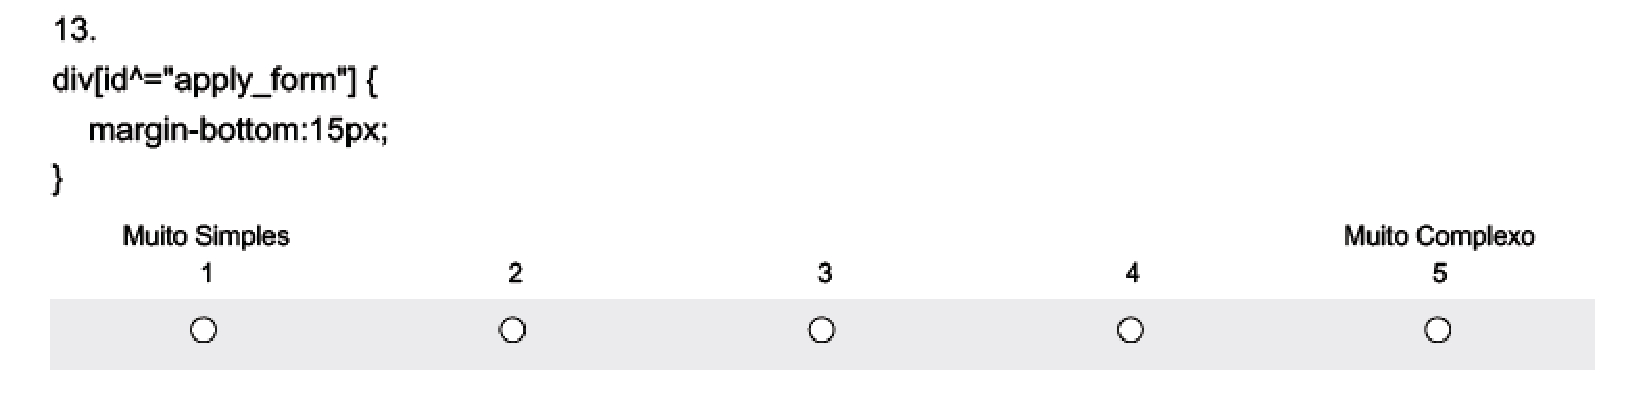
\includegraphics[width=1\textwidth]{./04-figuras/questionario_q13}
	\fonte{Próprio autor}
	\label{fig:questionario_q13}
\end{figure}

Viu-se necessária a avaliação da complexidade de alguns aspectos da linguagem a partir do ponto de vista do profissional. Para tal, o questionário (\autoref{chap:apendiceA}) foi construído com uma seção onde é avaliada, com base em um trecho de código (\autoref{fig:questionario_q13}), a dificuldade de se dar manutenção no mesmo. Cada trecho de código foi elaborado de acordo com um aspecto da linguagem que possa causar algum tipo de complicação. Esses aspectos foram escolhidos de acordo com as ponderações e experiência do autor, com base nos estudos realizados.

A dificuldade atribuída por cada pessoa a um determinado conjunto de regras e propriedades, é subjetiva e depende fortemente da experiência do indivíduo. Portanto, construiu-se o questionário com perguntas visando a classificação do respondente de acordo com o seu nível de conhecimento. A partir, dessa classificação foi possível ponderar as respostas de acordo com o nível de proficiência dos respondentes.

\section{Resultados do Questionário}

O questionário (\autoref{chap:apendiceA}) somou um total de 27 respostas. Este número de respostas pode ser atribuído ao alcance dos meios de divulgação, ou seja, não se fez uso de um canal de comunicação de uso da comunidade de desenvolvedores CSS. Mesmo com um pequeno número de respostas, pôde-se executar uma análise a partir dos resultados da pesquisa. 

Durante os estudos para construção do questionário foram levantas as seguintes hipóteses:

\begin{itemize}
	\item \textbf{(h0)} A manutenção de folhas de estilo não é um trabalho trivial, podendo ocorrer efeitos colaterais durante esta etapa;
	\item \textbf{(h1)} O tamanho da folha de estilo é inversamente proporcional à manutenibilidade;
	\item \textbf{(h2)} Seletores com alta especificidade prejudicam a manutenção da folha de estilo;
	\item \textbf{(h3)} O uso correto de classes, com nomes coerentes, pode ser benéfico para a manutenção;
	\item \textbf{(h4)} A herança de propriedade é um fator causador de efeitos colaterais na etapa de manutenção;
	\item \textbf{(h5)} Seletores de alta complexidade prejudicam na manutenção;
	\item \textbf{(h6)} Regras que não são comumente utilizadas na construção de código CSS podem dificultar a manutenção.
\end{itemize}

O questionário teve, então, o intuito de validar essas hipóteses, de modo a confirmá-las ou refutá-las, através de uma série de questões exploratórias, para identificar os aspectos mais abstratos de qualidade, e questões específicas, para identificar os aspectos estruturais da linguagem que representam maior dificuldade no período de manutenção. Para identificar a relevância das respostas do questionário, os respondentes foram agrupados por nível de proficiência.

\subsection{Nível de Proficiência}

A primeira questão do questionário (\autoref{chap:apendiceA}) foi desenvolvida com o intuito de classificar os conhecimentos de cada respondente, para assim determinar o seu nível de proficiência. Essa classificação permitiu que os pesos definidos por cada respondente fosse ponderado no resultado final do questionário.

Para esta classificação, utilizou-se os critérios apresentados no \autoref{quad:classVsProf}, que indica as funcionalidades do CSS quanto ao seu nível de proficiência. Essa categorização foi feita pelo autor com base na complexidade e na frequência de uso de certas funcionalidades da linguagem CSS.

\begin{quadro}
	\centering
	\caption{Classificação das características do CSS e nível de proficiência}
	\label{my-label}
	\begin{tabular}{|l|l|l|}
		\hline
		\textbf{Iniciante}                                                                         & \textbf{Imtermediário}                                                                                                             & \textbf{Avançado}                                                                        \\ \hline
		\begin{tabular}[c]{@{}l@{}}Localidade\\ Agrupamento\\ Aninhamento\\ Box Model\end{tabular} & \begin{tabular}[c]{@{}l@{}}Herança\\ Transformation\\ Transition\\ Pseudo classes\\ Pseudo elementos\\ Especificidade\end{tabular} & \begin{tabular}[c]{@{}l@{}}At-rules\\ Media queries\\ Animation e keyframes\end{tabular} \\ \hline
	\end{tabular}
	\fonte{Próprio autor}
\end{quadro}


Cada critério recebeu um peso de acordo com sua categoria, sendo 1, 2 e 3 os valores para iniciante, intermediário e avançado, respectivamente. Um respondente foi considerado iniciante se somasse 12 ou menos em suas respostas, intermediário para o respondente que somasse de 13 a 20, e avançado caso suas respostas somassem 21 ou mais. 
%Dessa forma não seria necessário que o respondente tivesse conhecimento sobre todas as regras para ser considerado avançado e também impede que o seja somente por conhecer as regras avançadas. 

\subsection{Visão Geral}

As respostas para o questionário formaram um conjunto de dados capaz de validar as hipóteses levantadas, não de forma definitiva, mas com dados suficientes para construção da métrica.

As questões propostas para identificar os aspectos de qualidade do código CSS identificaram resultados diversos. Como na \autoref{fig:questionario_q2}, pode-se verificar que mais de 90\% dos respondentes identificaram os elementos estruturais, a nomenclatura coerente para as classes e identificadores (\texttt{id}) como sendo imprescindíveis para qualidade da folha de estilo.

\begin{figure}[!htb]
	\centering
	\caption{Resultado da questão 2 do questionário \autoref{chap:apendiceA}.}
	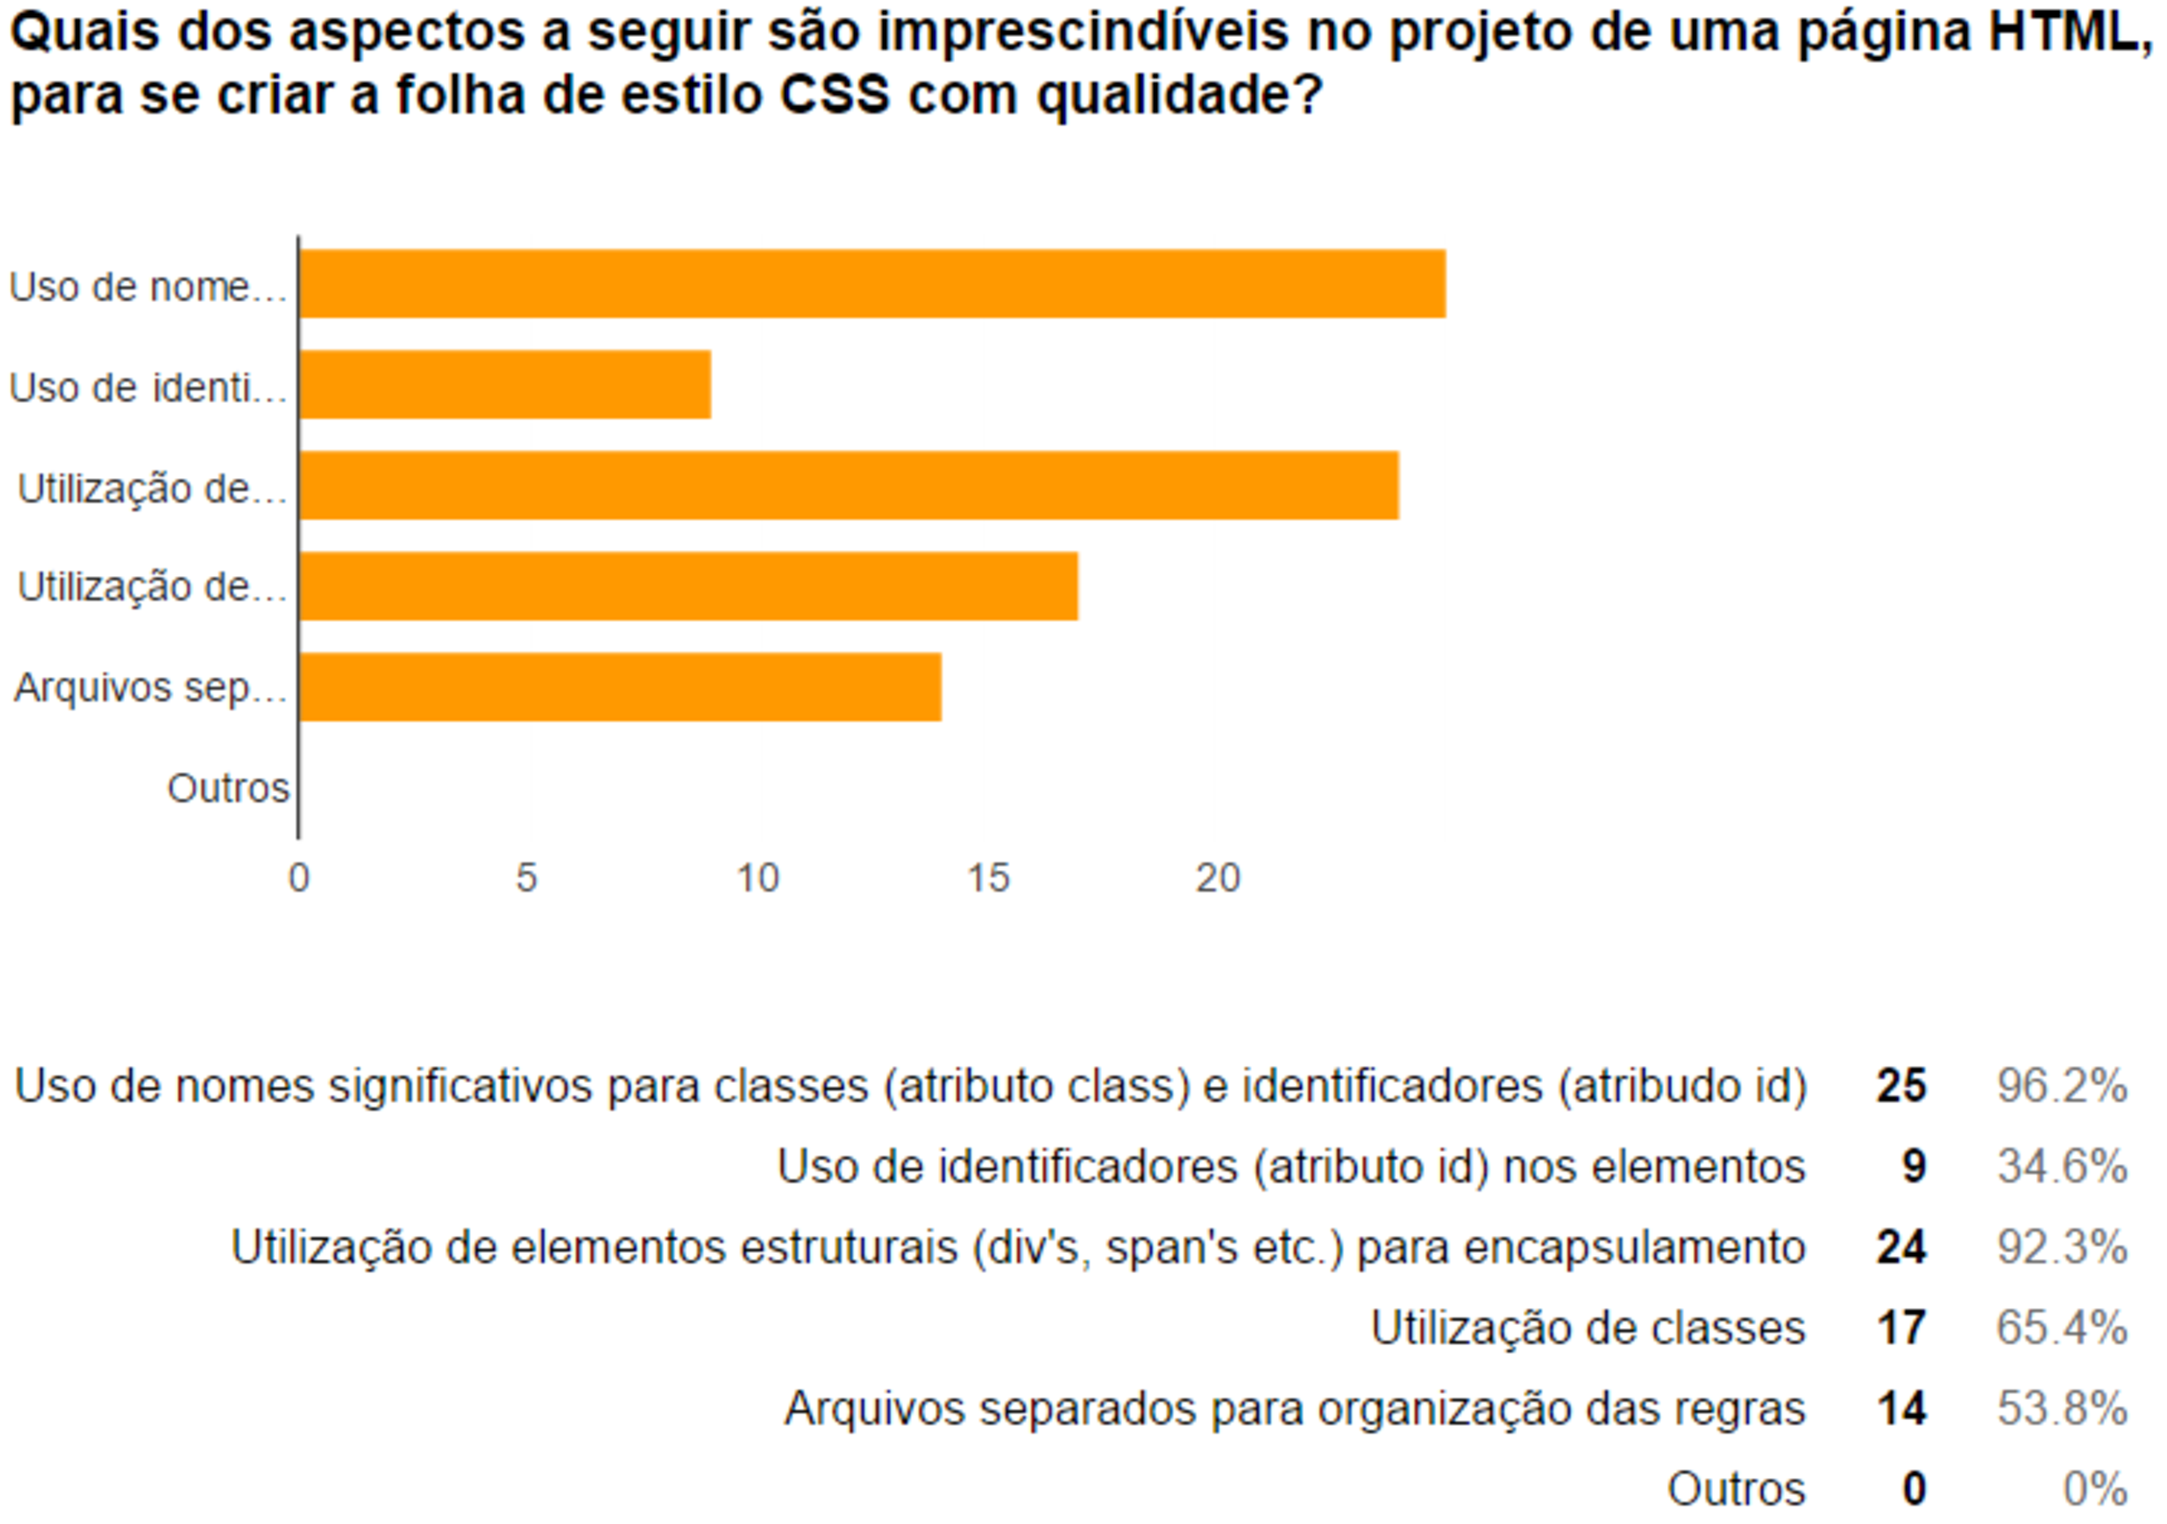
\includegraphics[width=1\textwidth]{./04-figuras/questionario_q2}
	\fonte{Próprio autor}
	\label{fig:questionario_q2}
\end{figure}

Essas respostas corroboram com a hipótese h3, mostrando que a boa estruturação dos elementos do documento de conteúdo, impactam diretamente na construção da folha de estilo.

Na questão exposta na \autoref{fig:questionario_q3}, pode-se notar os aspectos do CSS que interferem na qualidade do código. Nota-se aqui que não houve unanimidade para esta questão, porém percebe-se uma maior pontuação nas questões que têm impacto na legibilidade do código, \textit{e.g.} organização em seções e modularidade do código.

\begin{figure}[!htb]
	\centering
	\caption{Resultado da questão 3 do questionário \autoref{chap:apendiceA}.}
	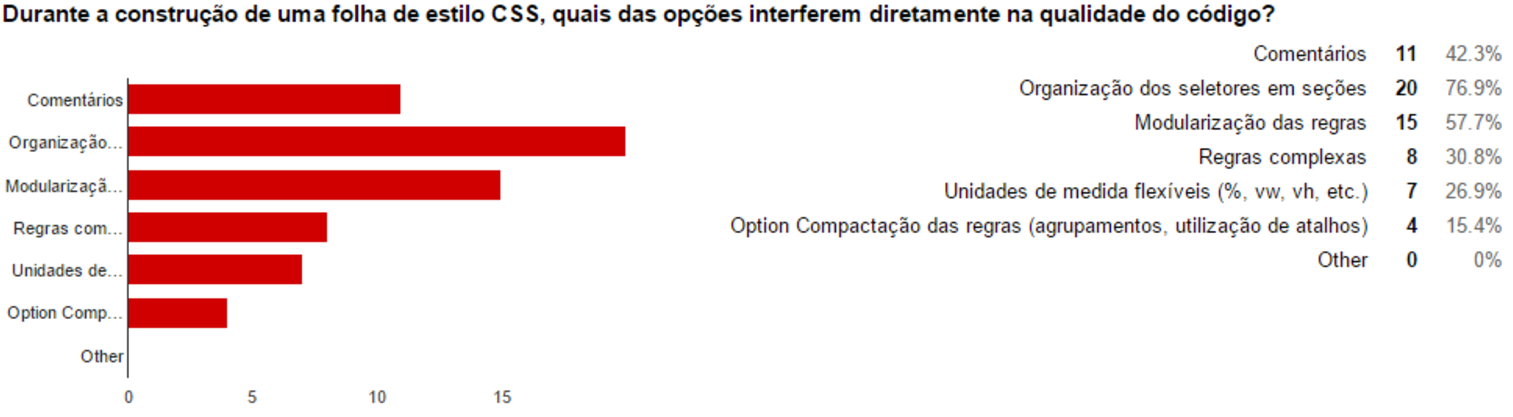
\includegraphics[width=1\textwidth]{./04-figuras/questionario_q3}
	\fonte{Próprio autor}
	\label{fig:questionario_q3}
\end{figure}

Na \autoref{fig:questionario_q9}, é possível verificar que o maior número de ocorrências de efeitos colaterais, para os respondentes, está na fase de manutenção do código. Esse resultado corrobora com a hipótese h0.

\begin{figure}[!htb]
	\centering
	\caption{Resultado da questão 9 do questionário \autoref{chap:apendiceA}.}
	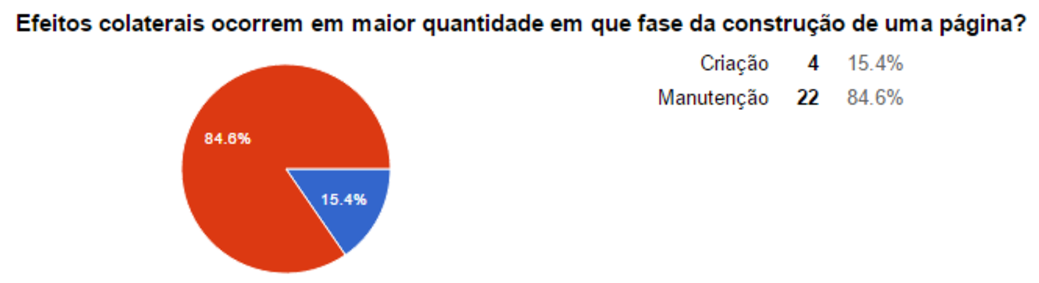
\includegraphics[width=1\textwidth]{./04-figuras/questionario_q9}
	\fonte{Próprio autor}
	\label{fig:questionario_q9}
\end{figure}

Ainda sobre os efeitos colaterais, foi elaborada uma questão com objetivo de identificar quais são as propriedades do CSS que mais os causam. As respostas foram variadas e por isso não foi possível identificar um padrão a partir desta pesquisa. No entanto, as respostas com elementos semelhantes sempre tinham relação com definição de posicionamento e tamanho dos elementos (e.g.: \texttt{position}, \texttt{margin}, \texttt{padding}, \texttt{display}, \texttt{width}, \texttt{z-index}, \texttt{float}, etc). A partir das respostas obtidas, pode-se identificar os valores de manutenibilidade para os elementos que possuírem características de herança, prioridade e atuação semelhantes.

\subsection{Questões Exploratórias}

Algumas questões desse questionário tinham o objetivo de captar informações da experiência dos respondentes, a fim de identificar parâmetros que não foram cobertos pelo questionário. Algumas respostas agregaram valor à pesquisa, identificando esses pontos e mostrando algumas informações valiosas acerca da qualidade da folha de estilo. 

Foi questionado quais são os pontos críticos que podem dificultar a manutenção, ou evolução, do código CSS. Das respostas obtidas, pode-se notar no \autoref{qd:openAnswers} aquelas que corroboram ou refutam as hipóteses levantadas.

\begin{quadro}[!htb]
	\centering
	\caption{Contribuição das respostas da questão 6 do questionário. (\autoref{chap:apendiceA})}
	\label{qd:openAnswers}
	\begin{tabular}{|l|c|c|}
		\hline
		\textbf{Resposta}                                                                                                                                                                                                                                                                                                                                                                                                                                                                                                            & \multicolumn{1}{l|}{\textbf{Corrobora}} & \multicolumn{1}{l|}{\textbf{Refuta}} \\ \hline
		Estilizar elementos sem classe, criar folhas de estilos muito extensas.                                                                                                                                                                                                                                                                                                                                                                                                                                                      & h1                                      &                                      \\ \hline
		CSS's que são atribuídos de forma mais genérica aos elementos.                                                                                                                                                                                                                                                                                                                                                                                                                                                                &                                         & h2                                   \\ \hline
		\begin{tabular}[c]{@{}l@{}}Regras complexas \\ Herança de valor de propriedade (valores,inherit, initial)\\ Aninhamento (seleção de elementos aninhados)\end{tabular}                                                                                                                                                                                                                                                                                                                                                  & h5                                      &                                      \\ \hline
		\begin{tabular}[c]{@{}l@{}}Utilização de nomes muitos genéricos para classes ou atributos.\\ A estilização que não é mais usada e fica no código.\end{tabular}                                                                                                                                                                                                                                                                                                                                                               & h3;h6                                   &                                      \\ \hline
		\begin{tabular}[c]{@{}l@{}}Regras para itens muito genéricos. \\ Utilização de !imporant. \\ Código repetido.\end{tabular}                                                                                                                                                                                                                                                                                                                                                                                                   & h6                                      & h2                                   \\ \hline
		Saber se um seletor está ou não sendo usado em algum parte do código.                                                                                                                                                                                                                                                                                                                                                                                                                                                        & h6                                      &                                      \\ \hline
		Seletores muito específicos.                                                                                                                                                                                                                                                                                                                                                                                                                                                                                                  & h2                                      &                                      \\ \hline
		\begin{tabular}[c]{@{}l@{}}Regras com seletores muito gerais, como classes e tags, \\ costumam provocar efeitos colaterais com mais frequência.\\ Acho que para poder escrever regras desse tipo (gerais), \\ todas as propriedades sendo definidas precisam ser "óbvias" \\ (fácil de uma 3ª pessoa entender por que ela está ali) \\ e também gerais (não sendo algo como uma classe .button \\ definindo um left:54px, que deveria estar sendo aplicado \\ a apenas um .button em particular e não a todos).\end{tabular} & h2                                      &                                      \\ \hline
		\begin{tabular}[c]{@{}l@{}}Arquivo desorganizado, regras repetidas, \\ sem sessões definidas,código compactado.\end{tabular}                                                                                                                                                                                                                                                                                                                                                                                                  & h3;h6                                   &                                      \\ \hline
	\end{tabular}
	\fonte{Próprio autor, a partir de respostas do questionário}
\end{quadro}

Essas respostas foram de suma importância para identificação de quais os critérios que deveriam, ou não, ser considerados para a avaliação da folha de estilo. Depois de identificados esses critérios, foi feita a análise das questões com exemplos de código, com o objetivo de definir os seus pesos.

\subsection{Cálculo dos Pesos}

A última seção de perguntas no questionário foi desenvolvida com a intenção de identificar as dificuldades dos respondentes, quando deparados com uma situação em que precisariam modificar um trecho de código CSS. As propriedades e regras exemplificadas foram desenvolvidas com objetivos específicos, cada uma delas cobrindo uma das características que representavam, na visão do autor, um fator dificultador na modificação de uma folha de estilo.

Cada respondente identificou em uma escala (1 a 5) a dificuldade de se dar manutenção no trecho de código apresentado. Fez-se, então, uma média dos valores atribuídos pelos respondentes para cada resposta, para determinar o grau de dificuldade de alterar os 16 trechos de código CSS representando as diferentes características da linguagem. Pode-se notar na \autoref{fig:graph_scaleMean} a diferença de dificuldade encontrada pelos respondentes com diferentes níveis de proficiência.

\begin{figure}[!htb]
	\centering
	\caption{Média de dificuldade por nível de proficiência em cada uma das questões de escala.}
	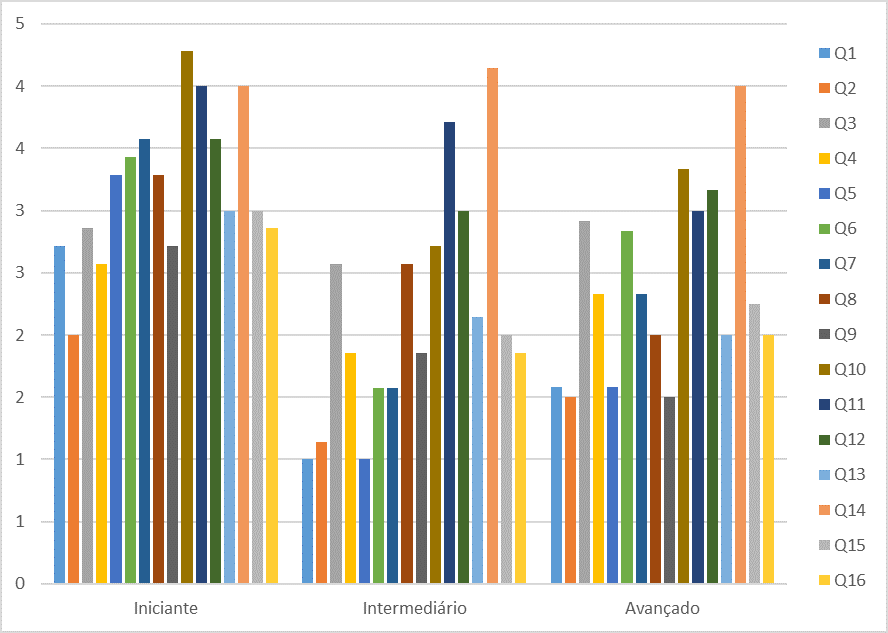
\includegraphics[width=1\textwidth]{./04-figuras/graph_scaleMean}
	\fonte{Próprio autor}
	\label{fig:graph_scaleMean}
\end{figure}

É possível notar a proximidade das respostas dos níveis intermediário e avançado, mas ainda assim as médias do nível avançado são ligeiramente maiores que as do nível intermediário. Os pesos de cada critério foi identificado a partir da média ponderada de cada questão, para evitar que o peso de cada resposta fosse completamente dependente das respostas dos respondentes identificados como iniciantes.

\section{Criação da Métrica}
	
A partir das hipóteses levantadas e dos resultados obtidos no questionário, foram identificados 12 aspectos da linguagem a serem avaliados e, a partir deles, foram elaborados os critérios utilizados para o cálculo da métrica. O peso para cada um dos critérios de avaliação foi, então, definido a partir dos resultados obtidos no questionário, como visto na \autoref{tab:tabelaPesos}. Esses pesos foram utilizados para o cálculo de cada métrica de forma individual, aplicando uma forma de avaliação correspondente a cada um dos critérios.

\begin{table}[!htb]
	\centering
	\caption{Tabela com peso de cada critério avaliado.}
	\label{tab:tabelaPesos}
	\begin{tabular}{l|l}
		\textbf{Critério}                                                           & \textbf{Peso} \\ \hline
		Seletores raros: \{{[}\textasciicircum ={]}, {[}\$={]}, \char`~, +,\textgreater\} & 3             \\
		Agrupamentos                                                                & 2,8           \\
		Aninhamento                                                                 & 2,8           \\
		Propriedade simplificada                                                    & 3,2           \\
		Pseudo elementos                                                            & 2,8           \\
		Seletor com mais de 35 caracteres                                           & 3             \\
		At-rules                                                                    & 2,8           \\
		Media queries                                                               & 3,8           \\
		Prefixos: \{-webkit, -ms, etc.\}                                            & 4,2           \\
		Clausula :not                                                               & 3,8           \\
		Complexidade do seletor                                                     & 4,8           \\
		Seletor de localidade: \{nth-last-child, first-child, etc.\}                & 2,6          
	\end{tabular}
	\fonte{Próprio autor}
\end{table}

\subsection{Identificação dos Critérios de Avaliação}
  
%Mostrar e explicar o mapeamento de cada questão de trecho de código com sua respectiva funcionalidade.
Cada uma das 16 questões teve o objetivo de avaliar um aspecto da linguagem com o intuito de direcionar a escolha dos critérios de avaliação. Portanto fez-se uma mapeamento das funcionalidades abordadas em cada questão e, a partir disso, determinou-se os critérios que seriam avaliados pelo \textit{script} de cálculo da métrica.

Como pode ser visto no \autoref{quad:questionXfunc}, as funcionalidades abordadas por cada uma das questões específicas foram definidas pelo próprio autor, de acordo com a sua experiência em codificação CSS, como sendo as funcionalidades que impactam, de alguma forma, na manutenibilidade do código.

\begin{quadro}[]
\centering
\caption{Quadro com as funcionalidades exploradas em cada questão do questionário no \autoref{chap:apendiceA}}
\label{quad:questionXfunc}
\begin{tabular}{|c|l|}
\hline
\textbf{Questão} & \textbf{Funcionalidade}                                                  \\ \hline
Q1               & Seletor de classe simples                                                \\ \hline
Q2               & Seletor de id simples                                                    \\ \hline
Q3               & Pseudo seletor de substring (\textasciicircum =)                         \\ \hline
Q4               & Agrupamento de seletores                                                 \\ \hline
Q5               & Pseudo classe                                                            \\ \hline
Q6               & Propriedades simplificadas                                               \\ \hline
Q7               & Pseudo elemento                                                          \\ \hline
Q8               & Seletor muito longo                                                      \\ \hline
Q9               & At-rule                                                                  \\ \hline
Q10              & Media queries                                                            \\ \hline
Q11              & Seletores com webkit, utilizando propiedades de webkit                   \\ \hline
Q12              & Uso da clausula not                                                      \\ \hline
Q13              & Child selector                                                           \\ \hline
Q14              & Seletor de alta complexidade: localização + sibling  + seletor universal \\ \hline
Q15              & Conflito de herança na cor da tag b                                      \\ \hline
Q16              & Seletor de localidade: first-child                                       \\ \hline
\end{tabular}
\end{quadro}

A partir dessas funcionalidades foram identificados quais os métodos de avaliação caberiam a cada um deles. Esses métodos foram denominados critérios, que, para o \textit{script} de cálculo, representam um padrão a ser identificado, contado e calculado. Desta forma foram definidos e construídos os critérios listados na \autoref{tab:tabelaPesos}.

Cada um dos critérios criados representa um impacto na qualidade, esse impacto foi definido como sendo o peso do critério avaliado. Dessa forma o \textit{script} avalia a presença ou não de cada critério nas regras definidas na folha de estilo CSS e, então, para cada ocorrência soma-se o peso do critério ao total da métrica. Pode-se considerar como sendo a forma geral o que se define na \autoref{math:criteria}

\begin{equation}
\label{math:criteria}
	crit\acute{e}rio(regra) \rightarrow \# ocorr\hat{e}ncias * peso
\end{equation}

Em seguida foi definido como cada critério impacta na manutenibilidade, explicando em detalhe o funcionamento de cada um.

\subsubsection{Seletores Raros}
Os seletores definidos como raros, para este critério, foram identificados a partir da experiência do autor. Os seletores escolhidos foram: o seletor de atributo (\texttt{[attr=value]}); de descendente direto (\texttt{>}); de elementos irmãos (\texttt{\char`~}) e o de primeiro elemento irmão (\texttt{+}). O uso destes seletores nas regras CSS podem dificultar na manutenção, pois podem não ser de fácil entendimento, aumentando a complexidade do código e impactando assim na manutenibilidade.

A participação deste seletor na métrica foi calculada a partir da regra geral, identificando a repetição deste seletor em uma única regra e a frequência ao longo da folha de estilo. Nos testes executados este seletor teve pouca participação na métrica, o que corrobora com a premissa de que estes seletores são raramente utilizados.

\subsubsection{Agrupamento de elementos}
O agrupamento de seletores é identificado por regras que são aplicados a elementos distintos, ela é representada pela separação por virgulas e é muito utilizada pelos desenvolvedores. Para o cálculo desta métrica foi feito, então, uma contagem de seletores separados por virgula para cada regra avaliada, porém, identificou-se que há um limite no impacto que um agrupamento muito extenso pode causar. 

Devido ao limite identificado, foi utilizada uma função que mapeia o valor do critério em função do número de seletores agrupados na regra. Como podemos ver na \autoref{math:groupCriteria}, o limite de seletores agrupados é definido pelo denominador da função arco tangente, parâmetro este que foi ajustado para adequar aos testes executados.

\begin{equation}
\label{math:groupCriteria}
	crit\acute{e}rio(regra) \rightarrow arctg\left(\frac{\#ocorr\hat{e}ncias}{20}\right)	
\end{equation}

\subsubsection{Seletores Aninhados}
Este critério foi desenvolvido para avaliar a profundidade dos seletores. Para tanto, foi necessária a contagem de espaços em branco entre seletores simples, este tipo de aninhamento pode ocorrer em várias combinações de seletores, \textit{e.g.}, durante o agrupamento de seletores pode ocorrer um seletor aninhado.

Para o cálculo de impacto deste seletor também foi utilizada a \autoref{math:groupCriteria}, considerando-se que existe um limite de impacto para a profundidade de um seletor. Após o cálculo individual de cada seletor, foi feita a soma de ocorrências durante a folha de estilo.

\subsubsection{Propriedades Simplificadas}
A simplificação das propriedades CSS são um atalho, que permitem que o desenvolvedor aplique todos os possíveis atributos a uma propriedade sem ter que declarar todos. Como podemos ver no exemplo da \autoref{fig:shorthand}, não há uma sequência lógica fácil de se identificar para a declaração dos valores dessas propriedades, o que pode dificultar na manutenção desse tipo de regra.

\begin{figure}[!htb]
	\centering
	\caption{Exemplo de propriedades simplificadas.}
	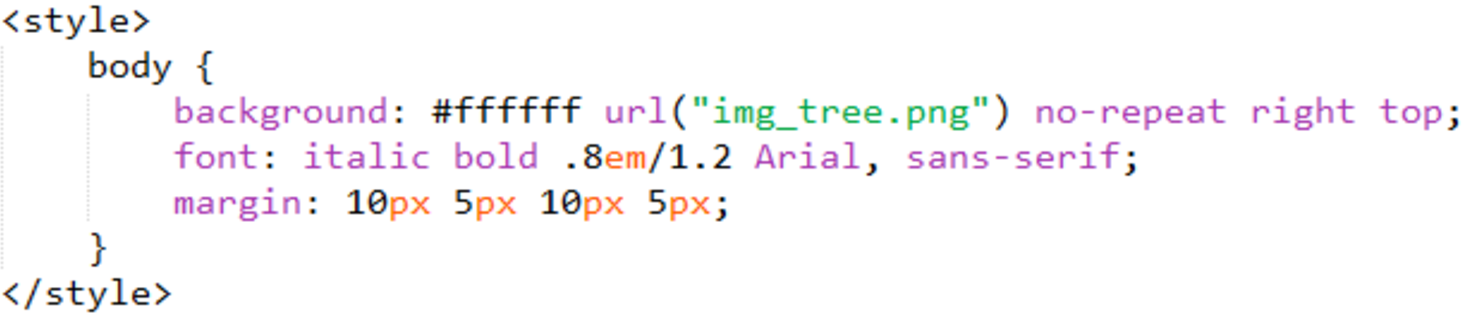
\includegraphics[width=1\textwidth]{./04-figuras/shorthand_prop}
	\fonte{Próprio autor}
	\label{fig:shorthand}
\end{figure}

Para calcular este critério foi identificadas as propriedades que possuíam valores atribuídos separados por espaço. Para cada propriedade contou-se o número de ocorrências e somou-se ao final. Seguindo o mesmo cálculo da \autoref{math:criteria}.

\subsubsection{Pseudo Elementos}
Os pseudo elementos podem ser utilizados para acessar propriedades especiais dos elementos HTML. Para este critério foram considerados os pseudo elementos e as pseudo classes em um único critério, uma vez que obtiveram a mesma média de dificuldade. Das pseudo classes foram excluídos a cláusula \texttt{not} e os seletores de localidade, que receberam um critério de avaliação separado.

O cálculo foi feito então de acordo com a ocorrência de pseudo elementos e pseudo classes presentes no seletor das regras, novamente avaliando em qualquer situação que esses possam aparecer. A participação deste critério é então medido como a frequência de ocorrências durante a folha de estilo.

\subsubsection{Comprimento de Seletores}
Para o cálculo do critério de comprimento dos seletores levou-se em consideração um valor de ativação, \textit{i.e.}, a partir de dado número de caracteres o seletor terá um valor de manutenibilidade. Para este valor de ativação utilizou-se dos dados levantados pela pesquisa feita por \citeonline{McPherson:2014}, em que são expostos alguns dados sobre a utilização do CSS na Internet. Nessa pesquisa, é apresentada uma distribuição do comprimento do seletor em caracteres. 

A distribuição na \autoref{fig:distributionLength}, mostra que a moda dos comprimentos encontrados pela pesquisa é em torno de 20 caracteres. A decisão tomada para o valor de ativação do critério foi então definida como 35 caracteres, um valor maior que a moda e que possui uma fatia expressiva na distribuição apresentada.

%mandar a figura pro xuxu que ele vai traduzir modafocka

\begin{figure}[!htb]
	\centering
	\caption{Distribuição de tamanho dos seletores}
	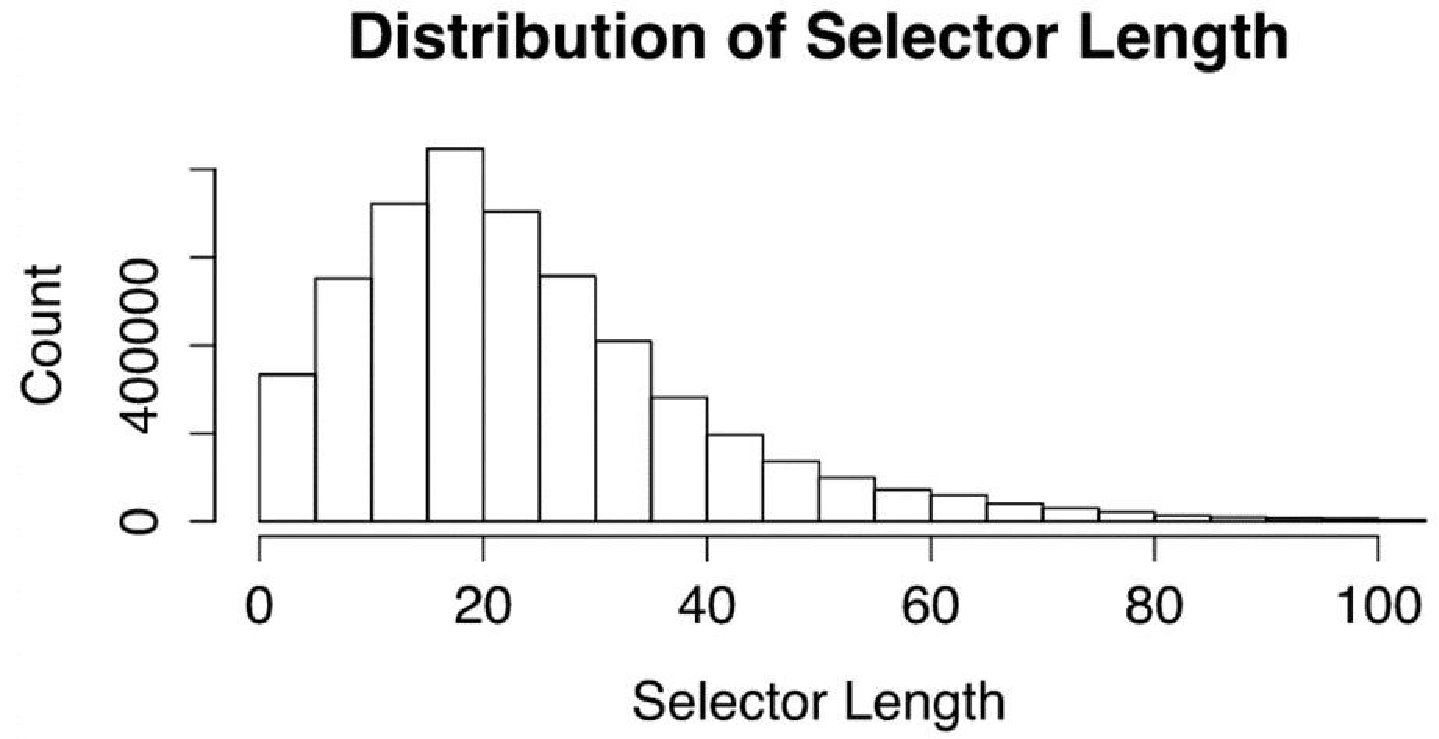
\includegraphics[width=0.8\textwidth]{./04-figuras/dist_selectorL}
	\fonte{\citeonline{McPherson:2014}}
	\label{fig:distributionLength}
\end{figure}

\subsubsection{\textit{At-rules}}
Este critério avaliou as \textit{At-rules}, denominadas assim por serem regras precedidas pelo símbolo @ (arroba). Esse critério foi calculado utilizando-se a \autoref{math:criteria}, contando o número de repetições ao longo da folha de estilo. As \textit{At-rules} podem definir uma série de atributos (\textit{e.g.} \texttt{charset}, \texttt{import}, \texttt{namespace}, etc.), que dão suporte à importação de arquivos externos ou o poder de controle condicional, como no caso do \texttt{@media}.

\subsubsection{\textit{Media Queries}}
A \textit{At-rule} \texttt{@media} é um caso especial do CSS, uma declaração que permite ao desenvolvedor implementar uma regra condicionada ao argumento chamado \textit{media querie}. As \textit{media queries} são condicionantes que avaliam aspectos da janela de renderização do HTML, ou informações do dispositivo no qual o HTML está sendo renderizado. As \textit{media queries} adicionam um nível a mais de complexidade no código CSS e tem ganhado espaço nas folhas de estilo devido à necessidade de estilos responsivos paras as páginas \textit{web}. 

As regras \texttt{@media} podem conter várias regras CSS condicionadas a suas \textit{media queries}, o que torna a avaliação mais complexa. Neste trabalho foi feito uma análise do número de \textit{media queries} presentes em cada arquivo CSS, cada uma avaliada como o peso determinado a elas na \autoref{tab:tabelaPesos} e somadas ao valor final da métrica.

Durante os testes no Jenkins, não foram encontradas \textit{media queries} muito complexas e elas só estavam presentes a partir da versão que exibia a preocupação com a estilização responsiva da aplicação. As regras eram relativamente simples e não houve grande participação para o resultado final dos testes.

\subsubsection{Prefixos}
Os prefixos são utilizados para explicitar como a máquina de renderização do navegador irá interpretar uma propriedade CSS. Apenas algumas propriedades têm a necessidade de se utilizar esses prefixos. Mas quando utilizados, eles resultam em uma repetição de propriedade, o que implica numa dificuldade de leitura e manutenção do código maior.

Esse critério fica, então, responsável por identificar o número de repetições destes prefixos e somar o peso de cada uma delas ao resultado final da métrica.

\subsubsection{Cláusula \texttt{:not}}
O critério de avaliação da cláusula \texttt{:not} foi separada das pseudo classes por determinar um fluxo lógico completamente diferente dos seletores em geral. Essa cláusula determina que o seletor que ele sucede não pode existir na árvore de seleção do DOM, \textit{i.e.}, serão selecionados os elementos que não possuírem o atributo negado em sua árvore DOM.

Essa inversão lógica pode causar um aumento na complexidade e deve ser, portanto, avaliada de forma exclusiva. Isto também pode ser identificado na \autoref{tab:tabelaPesos}, uma vez que o peso médio deste critério foi maior que o peso médio dos pseudo elementos e pseudo classes.

Esse critério calcula o número de ocorrências da cláusula \texttt{:not}, utilizando a forma geral e somando ao resultado final da métrica.

\subsubsection{Complexidade do Seletor}
Esse critério foi calculado de forma diferente, ele identifica uma combinação de seletores e calcula, a partir da presença dos símbolos \texttt{+}, \texttt{\char`~} e do identificador de propriedades \texttt{[attr=value]}, o valor da contribuição do critério como sendo o peso na \autoref{tab:tabelaPesos} potencializado pela quantidade de vezes que estes elementos aparecem.

\begin{equation}
\label{math:complexity}
	crit\acute{e}rio(regra) \rightarrow peso^{\#ocorr\hat{e}ncias}
\end{equation}

Como pode ser visto na \autoref{math:complexity}, o critério de complexidade tem crescimento exponencial, fazendo o dele o critério que deve se ter mais atenção. A complexidade dos seletores cresce de acordo com a necessidade de regras que não contam com os atributos \texttt{id} ou \texttt{class} do HTML, devido à dificuldade de se encontrar os atributos desejados dentro do DOM.

\subsection{\textit{Script} de Calculo Automático da Métrica}

Para fazer o cálculo da métrica de maneira automatizada, foi criado um \textit{script} que lê, a partir do DOM, as regras aplicadas sobre o HTML renderizado no navegador. Uma vez que o \textit{script} é executado no navegador, a versão de implementação do ECMAScript do navegador. Neste trabalho foi utilizado a versão 6 do ECMAScript, utilizando de algumas funções do JavaScript que não estão disponíveis em todos os navegadores.

Foram necessários alguns testes do \textit{script} para ajustes dos pesos e eles foram executados em várias páginas da \textit{web}.

\begin{figure}[!htb]
	\centering
	\caption{Exemplo de resultado da execução do \textit{script} de cálculo da métrica.}
	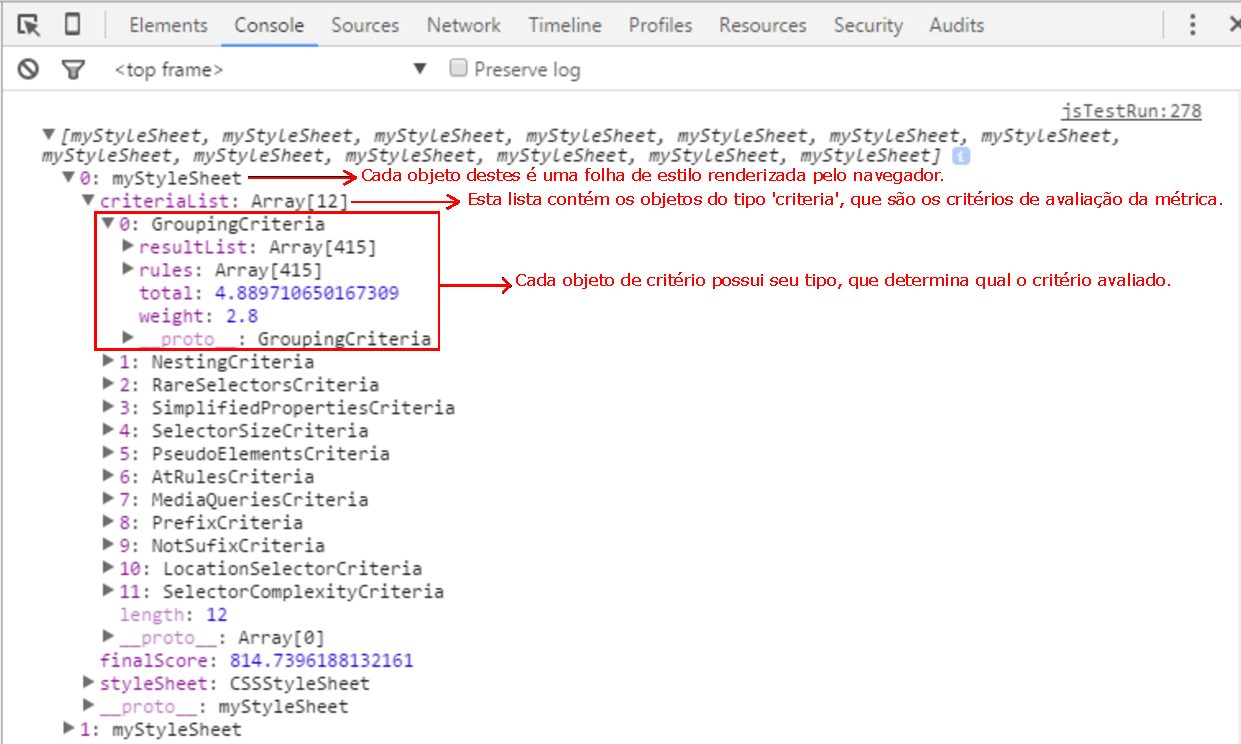
\includegraphics[width=1\textwidth]{./04-figuras/calculator}
	\fonte{Próprio autor}
	\label{fig:calculatorTest}
\end{figure}

O \textit{script} executa os cálculos de cada um dos critérios para cada folha de estilo renderizada, iterando sobre as regras CSS da folha de estilo. Dessa forma, uma mesma regra será avaliada sobre todos os critérios determinados, uma vez que as regras podem se encaixar em mais de um critério. Ao final da execução do \textit{script} é obtido o resultado total de cada critério em cada folha de estilo, o que permite uma análise da contribuição dos critérios para o resultado final da métrica.

Na \autoref{fig:calculatorTest}, pode-se visualizar a estrutura do resultado de uma execução do \textit{script}. O código fonte desse \textit{script} está disponível em um repositório no serviço gratuito de hospedagem de código aberto GitHub\footnote{Disponível em \url{https://github.com/vcsalvador/jsTestRun}.}. O objetivo final deste trabalho é gerar um \textit{bookmarklet}\footnote{Pequena aplicação construída em JavaScript para ser executada a partir do atalho de favoritos no navegador.\url{https://en.wikipedia.org/wiki/Bookmarklet}} que exiba as informações de qualidade do código CSS presente na página \textit{web}.

Com o \textit{script} para cálculo da métrica pronto e ajustado, fez-se a escolha de roteiro de testes. Para determinar qual seria a melhor forma de avaliar os resultados do \textit{script}, foi necessário escolher um projeto em que o estilo da página fosse codificado em arquivos CSS, eliminando a possibilidade de aplicar os testes em projetos que utilizem preprocessadores\footnote{Linguagens de programação intermediárias que geram código CSS, \textit{e.g.} Sass, Less, Stylus, etc.} CSS. Além desta limitação, deveria ser possível analisar um outro indicador de manutenibilidade de código, como tempo de evolução, número de defeitos ou algum índice de retrabalho.

\chapter{Avaliação da Métrica}

O Jenkins\footnote{Disponível em \url{https://jenkins-ci.org/}}, uma aplicação de integração contínua de código aberto, foi escolhido como objeto de estudo para avaliação da métrica por atender a todas as limitações identificadas. Ele é um projeto maduro, largamente utilizado e com uma comunidade de desenvolvimento ativa. Pode-se ver na \autoref{fig:codeFreqGraph} a quantidade de adições e exclusões de linha de código por semana, desde o ano de 2007. Ele também foi escolhido como objeto de estudo por utilizar somente código CSS para a construção de suas folhas de estilo.

\begin{figure}[!htb]
	\centering
	\caption{Gráfico de frequência de codificação do Jenkins.}
	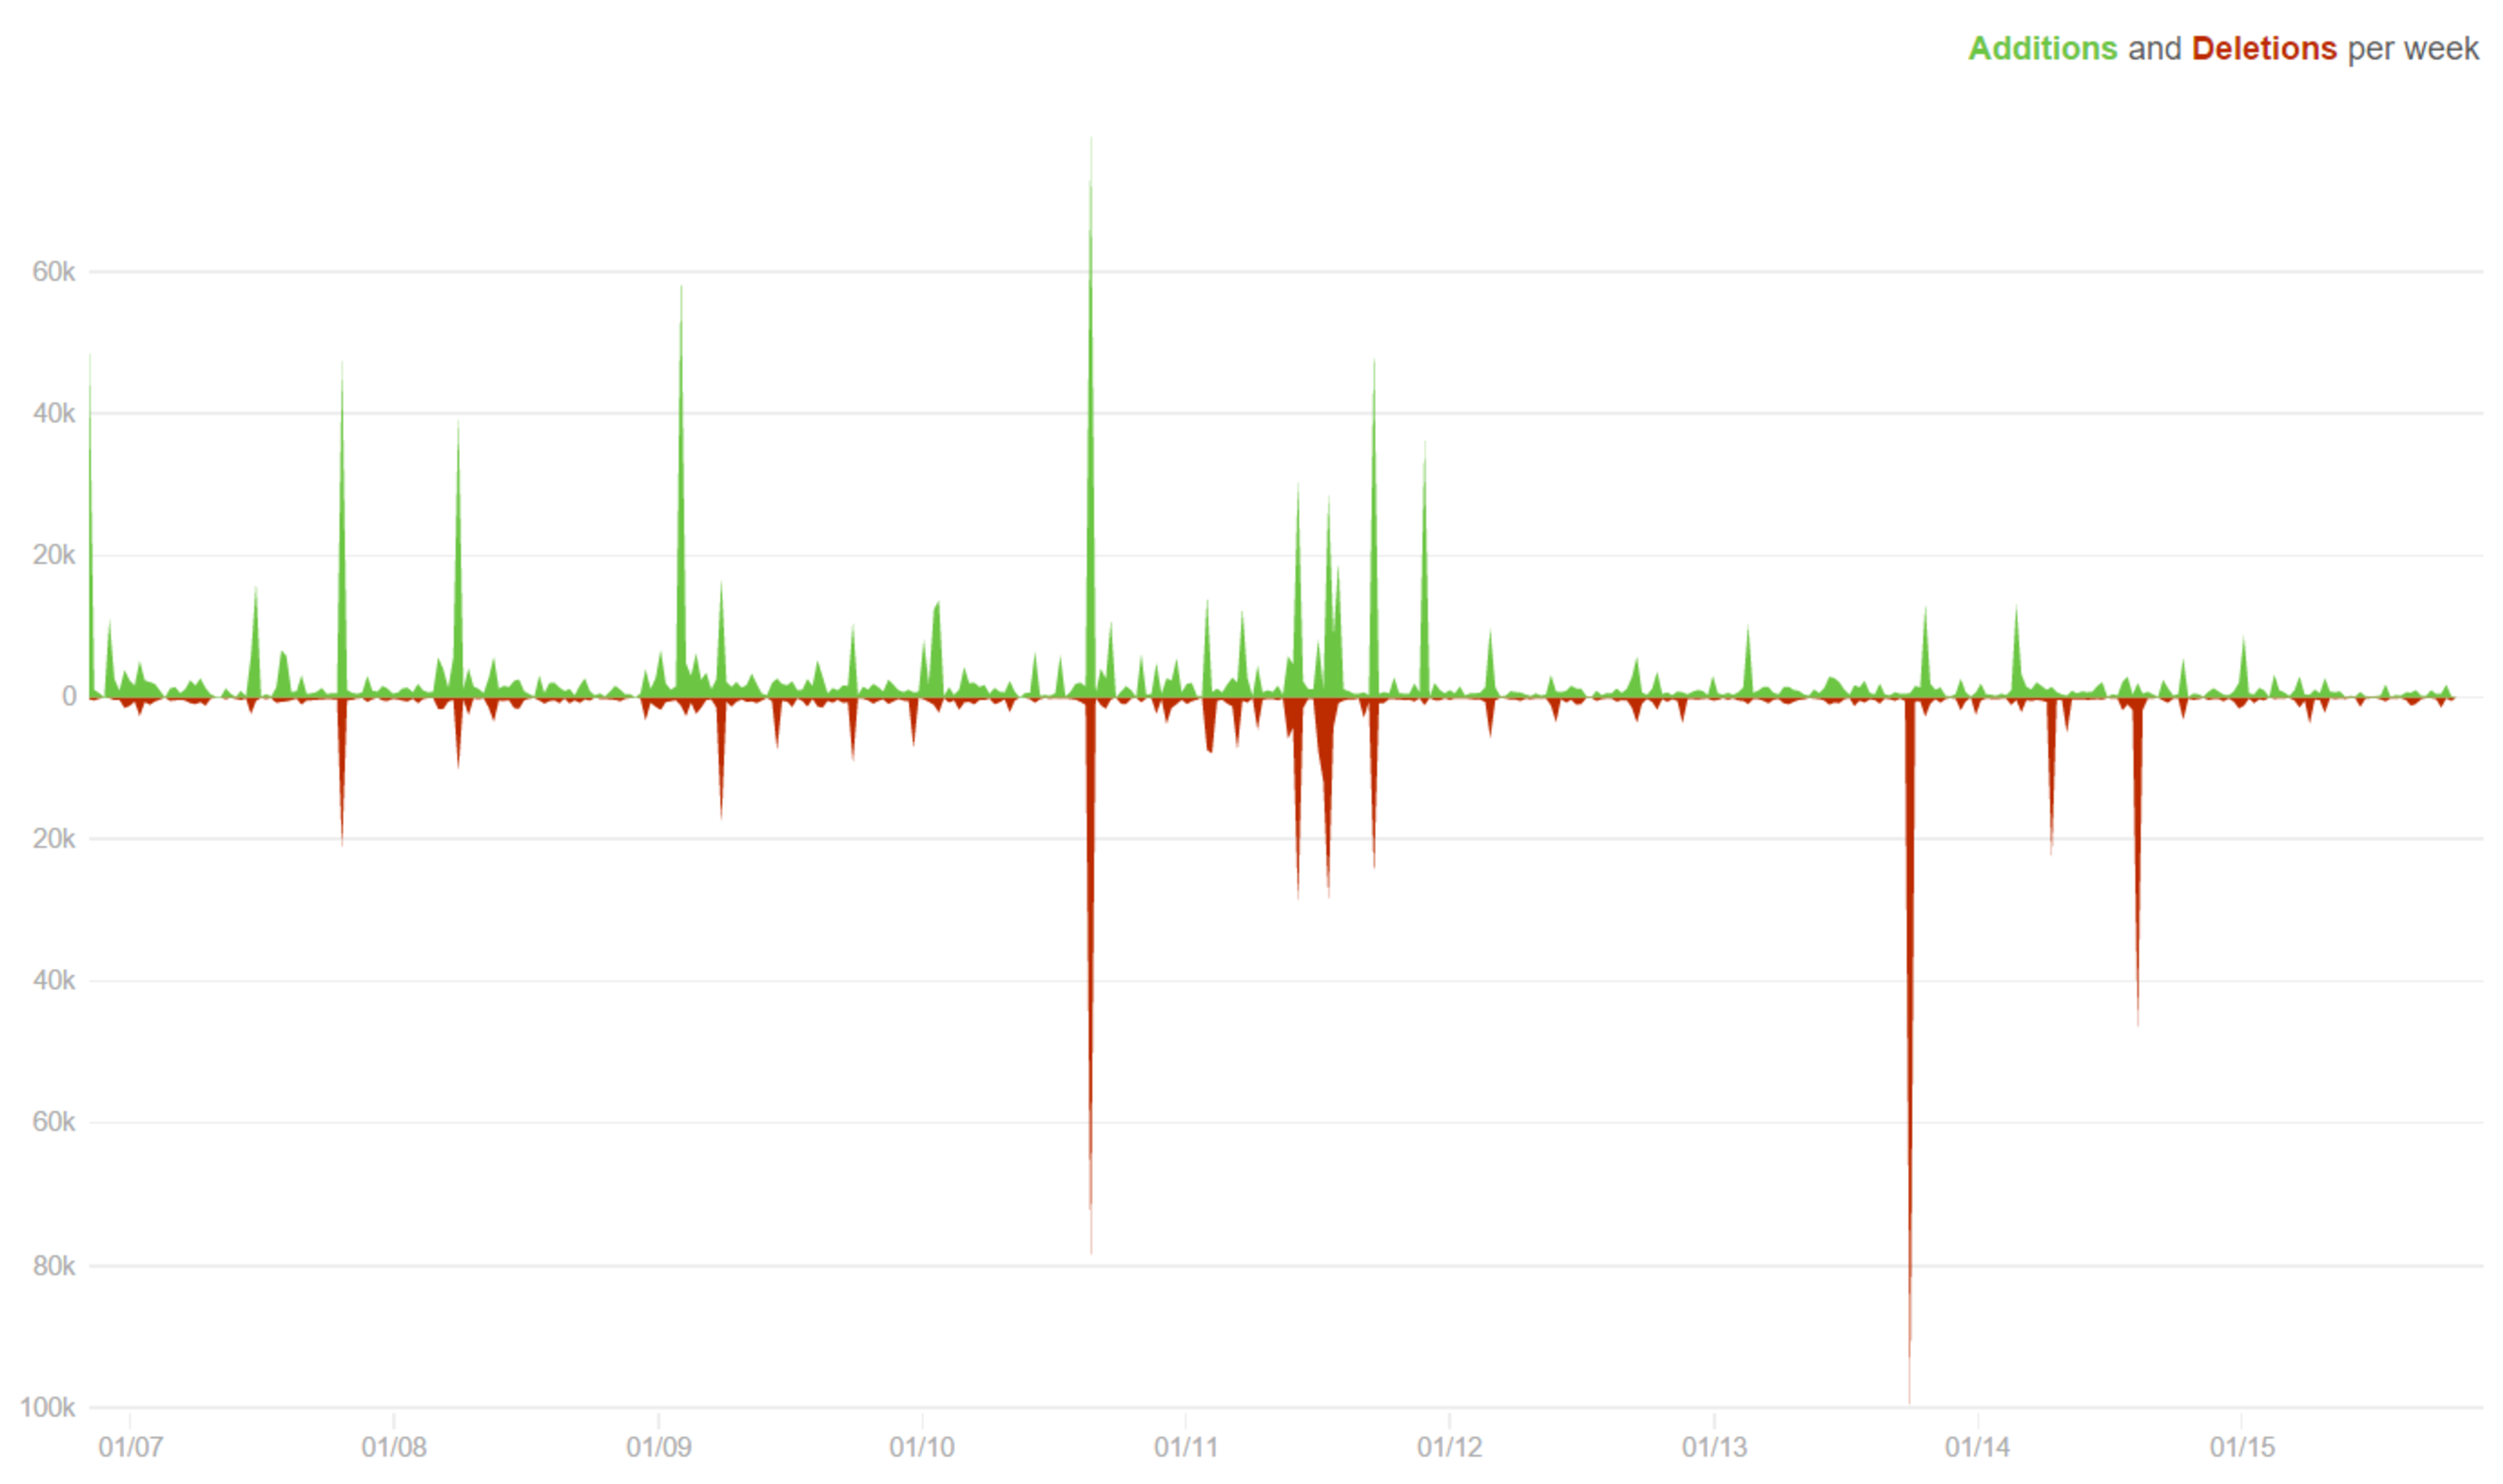
\includegraphics[width=1\textwidth]{./04-figuras/code_freq_graph}
	\fonte{GitHub, disponpível em \url{https://github.com/jenkinsci/jenkins/graphs/code-frequency}. Acessado em 24/10/2015.}
	\label{fig:codeFreqGraph}
\end{figure}

\section{Metodologia de Avaliação}

Para execução dos testes foi utilizado doze versões do Jenkins, selecionadas entre as que estão disponibilizadas para \textit{download} na página do projeto, em intervalos semestrais, para obter dados históricos da aplicação. Essas versões foram escolhidas entre 2010 até a versão mais atual, tendo essa escolha sido feita devido à disponibilidade e possibilidade de identificar em qual ponto no tempo elas foram construídas, conforme exibido no \autoref{tab:versionTabs}.

\begin{quadro}[]
	\centering
	\caption{Versões utilizadas para execução dos testes.}
	\label{tab:versionTabs}
	\begin{tabular}{|l|c|}
		\hline
		\textbf{Versão} & \textbf{Data de lançamento} \\ \hline
		1.369           & 31/07/2010            \\ \hline
		1.395           & 22/01/2011            \\ \hline
		1.423           & 25/07/2011            \\ \hline
		1.450           & 30/01/2012            \\ \hline
		1.475           & 01/08/2012            \\ \hline
		1.500           & 26/01/2013            \\ \hline
		1.525           & 29/07/2013            \\ \hline
		1.549           & 26/01/2014            \\ \hline
		1.574           & 27/07/2014            \\ \hline
		1.598           & 25/01/2015            \\ \hline
		1.622           & 27/07/2015            \\ \hline
		1.633           & 11/10/2015           \\ \hline
	\end{tabular}
	\fonte{Próprio autor}
\end{quadro}

%verificar comentários para este parágrafo... 

O projeto do Jenkins disponibiliza um meio de se cadastrar e controlar as tarefas relativas ao desenvolvimento da ferramenta JIRA\footnote{Disponível em \url{https://issues.jenkins-ci.org}}. Utilizando dos filtros disponíveis no JIRA, foi possível identificar as tarefas que tinham alguma relação com os arquivos CSS, tornando possível uma coleta de dados indicadores do período de manutenção do projeto. Devido às características do JIRA, não foi possível a coleta do tempo gasto em cada tarefa, então o indicador escolhido foi a quantidade de defeitos criados a partir da versão em teste no momento.

O filtro do JIRA foi configurado utilizando a ferramenta de busca avançada, onde a busca poderia ser feita em forma textual. O filtro foi construído com os filtros disponíveis pelo JIRA, buscamos dentro do projeto Jenkins pelos defeitos que possuíssem a etiqueta 'css' ou a palavra CSS dentro do texto de sua descrição, dessa forma pudemos identificar quais os defeitos do projeto estavam relacionados de alguma forma com CSS, mesmo que tivessem sido encontrados em outro lugar e possuíssem algum detalhe de CSS relacionados.

O alcance dos defeitos foi escolhido a partir de suas datas de criação, os criados a partir da versão em teste até a data de lançamento da versão que seria testada a seguir, no caso da versão mais atual foi feito de sua data de lançamento até o dia em que a pesquisa foi realizada. O filtro foi construído de maneira textual, utilizando a sintaxe do JIRA, e se parece com o seguinte: project = JENKINS AND issuetype = Bug AND (labels = css OR text ~ CSS) AND (createdDate >= "2010/07/31" AND createdDate < "2011/01/22") ORDER BY created ASC. Os resultados dessa busca podem ser vistos no \autoref{quad:quadVersionBugs}.

Com estas informações é possível identificar uma relação entre o valor da métrica e o número de defeitos de cada versão e, a partir disso, averiguar se o valor da métrica proposta para um arquivo CSS (ou conjunto de arquivos) indica o nível de manutenibilidade desse(s) arquivo(s).

\section{Dados para Teste}

A partir do repositório de versões\footnote{Disponível em \url{https://updates.jenkins-ci.org/download/war/}} do Jenkins, selecionou-se algumas de forma a cobrir uma janela de tempo semestral para as avaliações.

Instâncias do Jenkins foram configuradas e executadas localmente para cada versão selecionada e, para cada uma foi executado o \textit{script} de cálculo automatizado da métrica para identificar o valor. Então, o valor encontrado de cada versão foi transcrito para uma planilha, contendo os resultados dos critérios para cada arquivo CSS encontrado pelo \textit{script} e o número de defeitos encontrados pelo filtro do JIRA, entre a data de lançamento da versão sendo testada no momento e a seguinte.

%mostrar visualmente para os macacos que não entendem oq eu to dizendo... todo mundo hauhauhauhauahuaha

O valor da métrica foi então calculado como sendo o somatório dos resultados de todos os critérios de cada arquivo. %O valor total da métrica encontrado para a página \textit{web} é o somatório da métrica de todos os arquivos.
Para os testes na página principal da aplicação, identificou-se mais de um arquivo que compunham o estilo da página. Junto a esses arquivos encontrou-se arquivos de uma biblioteca de componentes chamada YUI\footnote{Disponível em \url{http://yuilibrary.com/}} que é formada por arquivos JavaScript e CSS. Os arquivos pertencentes a essa biblioteca influenciam os resultados das métricas e certamente na manutenibilidade do CSS da aplicação.

\begin{table}[!htb]
	\scalefont{0.8}
	\centering
	\caption{Tabela com os resultados do \textit{script} de cálculo automático para a versão 1.369}
	\label{tab:explResultTestes}
	\begin{tabular}{l|c|c|c|c|c}
		\multicolumn{1}{c|}{\textbf{Critério}} & \textbf{style.css} & \textbf{container.css} & \textbf{yui-skin.css} & \textbf{yui-container.css} & \textbf{yui-menu.css} \\ \hline
		\textbf{Grouping}                      & 2,4614             & 0,6994                 & 33,2557               & 1,2575                     & 2,0847                \\ \hline
		\textbf{Nesting}                       & 16,8729            & 6,6957                 & 308,5058              & 12,2259                    & 11,2661               \\ \hline
		\textbf{Rare Selector}                 & 18,0000            & 0,0000                 & 9,0000                & 0,0000                     & 9,0000                \\ \hline
		\textbf{Simplified Properties}         & 0,0000             & 0,0000                 & 0,0000                & 0,0000                     & 0,0000                \\ \hline
		\textbf{Selector Size}                 & 81,0000            & 39,0000                & 1881,0000             & 78,0000                    & 90,0000               \\ \hline
		\textbf{Pseudo Elements}               & 61,6000            & 5,6000                 & 123,2000              & 0,0000                     & 5,6000                \\ \hline
		\textbf{At Rules}                      & 0,0000             & 0,0000                 & 0,0000                & 0,0000                     & 0,0000                \\ \hline
		\textbf{Media Queries}                 & 0,0000             & 0,0000                 & 0,0000                & 0,0000                     & 0,0000                \\ \hline
		\textbf{Prefix}                        & 0,0000             & 0,0000                 & 0,0000                & 0,0000                     & 0,0000                \\ \hline
		\textbf{Not Sufix}                     & 0,0000             & 0,0000                 & 0,0000                & 0,0000                     & 0,0000                \\ \hline
		\textbf{Location Selector}             & 8,4000             & 0,0000                 & 0,0000                & 0,0000                     & 0,0000                \\ \hline
		\textbf{Selector Complexity}           & 0,0000             & 0,0000                 & 0,0000                & 0,0000                     & 0,0000               
	\end{tabular}
	\fonte{Próprio autor}
\end{table}

Os resultados da métrica para os arquivos da biblioteca YUI foram destoantes em relação aos vistos nos arquivos que realmente foram codificados pela equipe de desenvolvimento, como pode ser visto na \autoref{tab:explResultTestes}. Apesar desta grande diferença de pontuação, foi necessário  analisar o resultado do agregado para construir uma análise da pontuação das folhas de estilo CSS carregadas na tela principal da aplicação, portanto incluindo os arquivos da biblioteca.

\section{Resultados}

%versões de teste é confuso e ver comentários
Como as versões para execução do cálculo da métrica foram escolhidas com intervalos semestrais, considerou-se a média dos resultados como o valor médio para cada ano. Foi feito, então, um cruzamento do valor médio obtido para cada ano com o número de defeitos criados no mesmo ano.

\begin{figure}[!htbp]
	\centering
	\caption{Comparação do resultado total da métrica em relação ao número de defeitos criados.}
	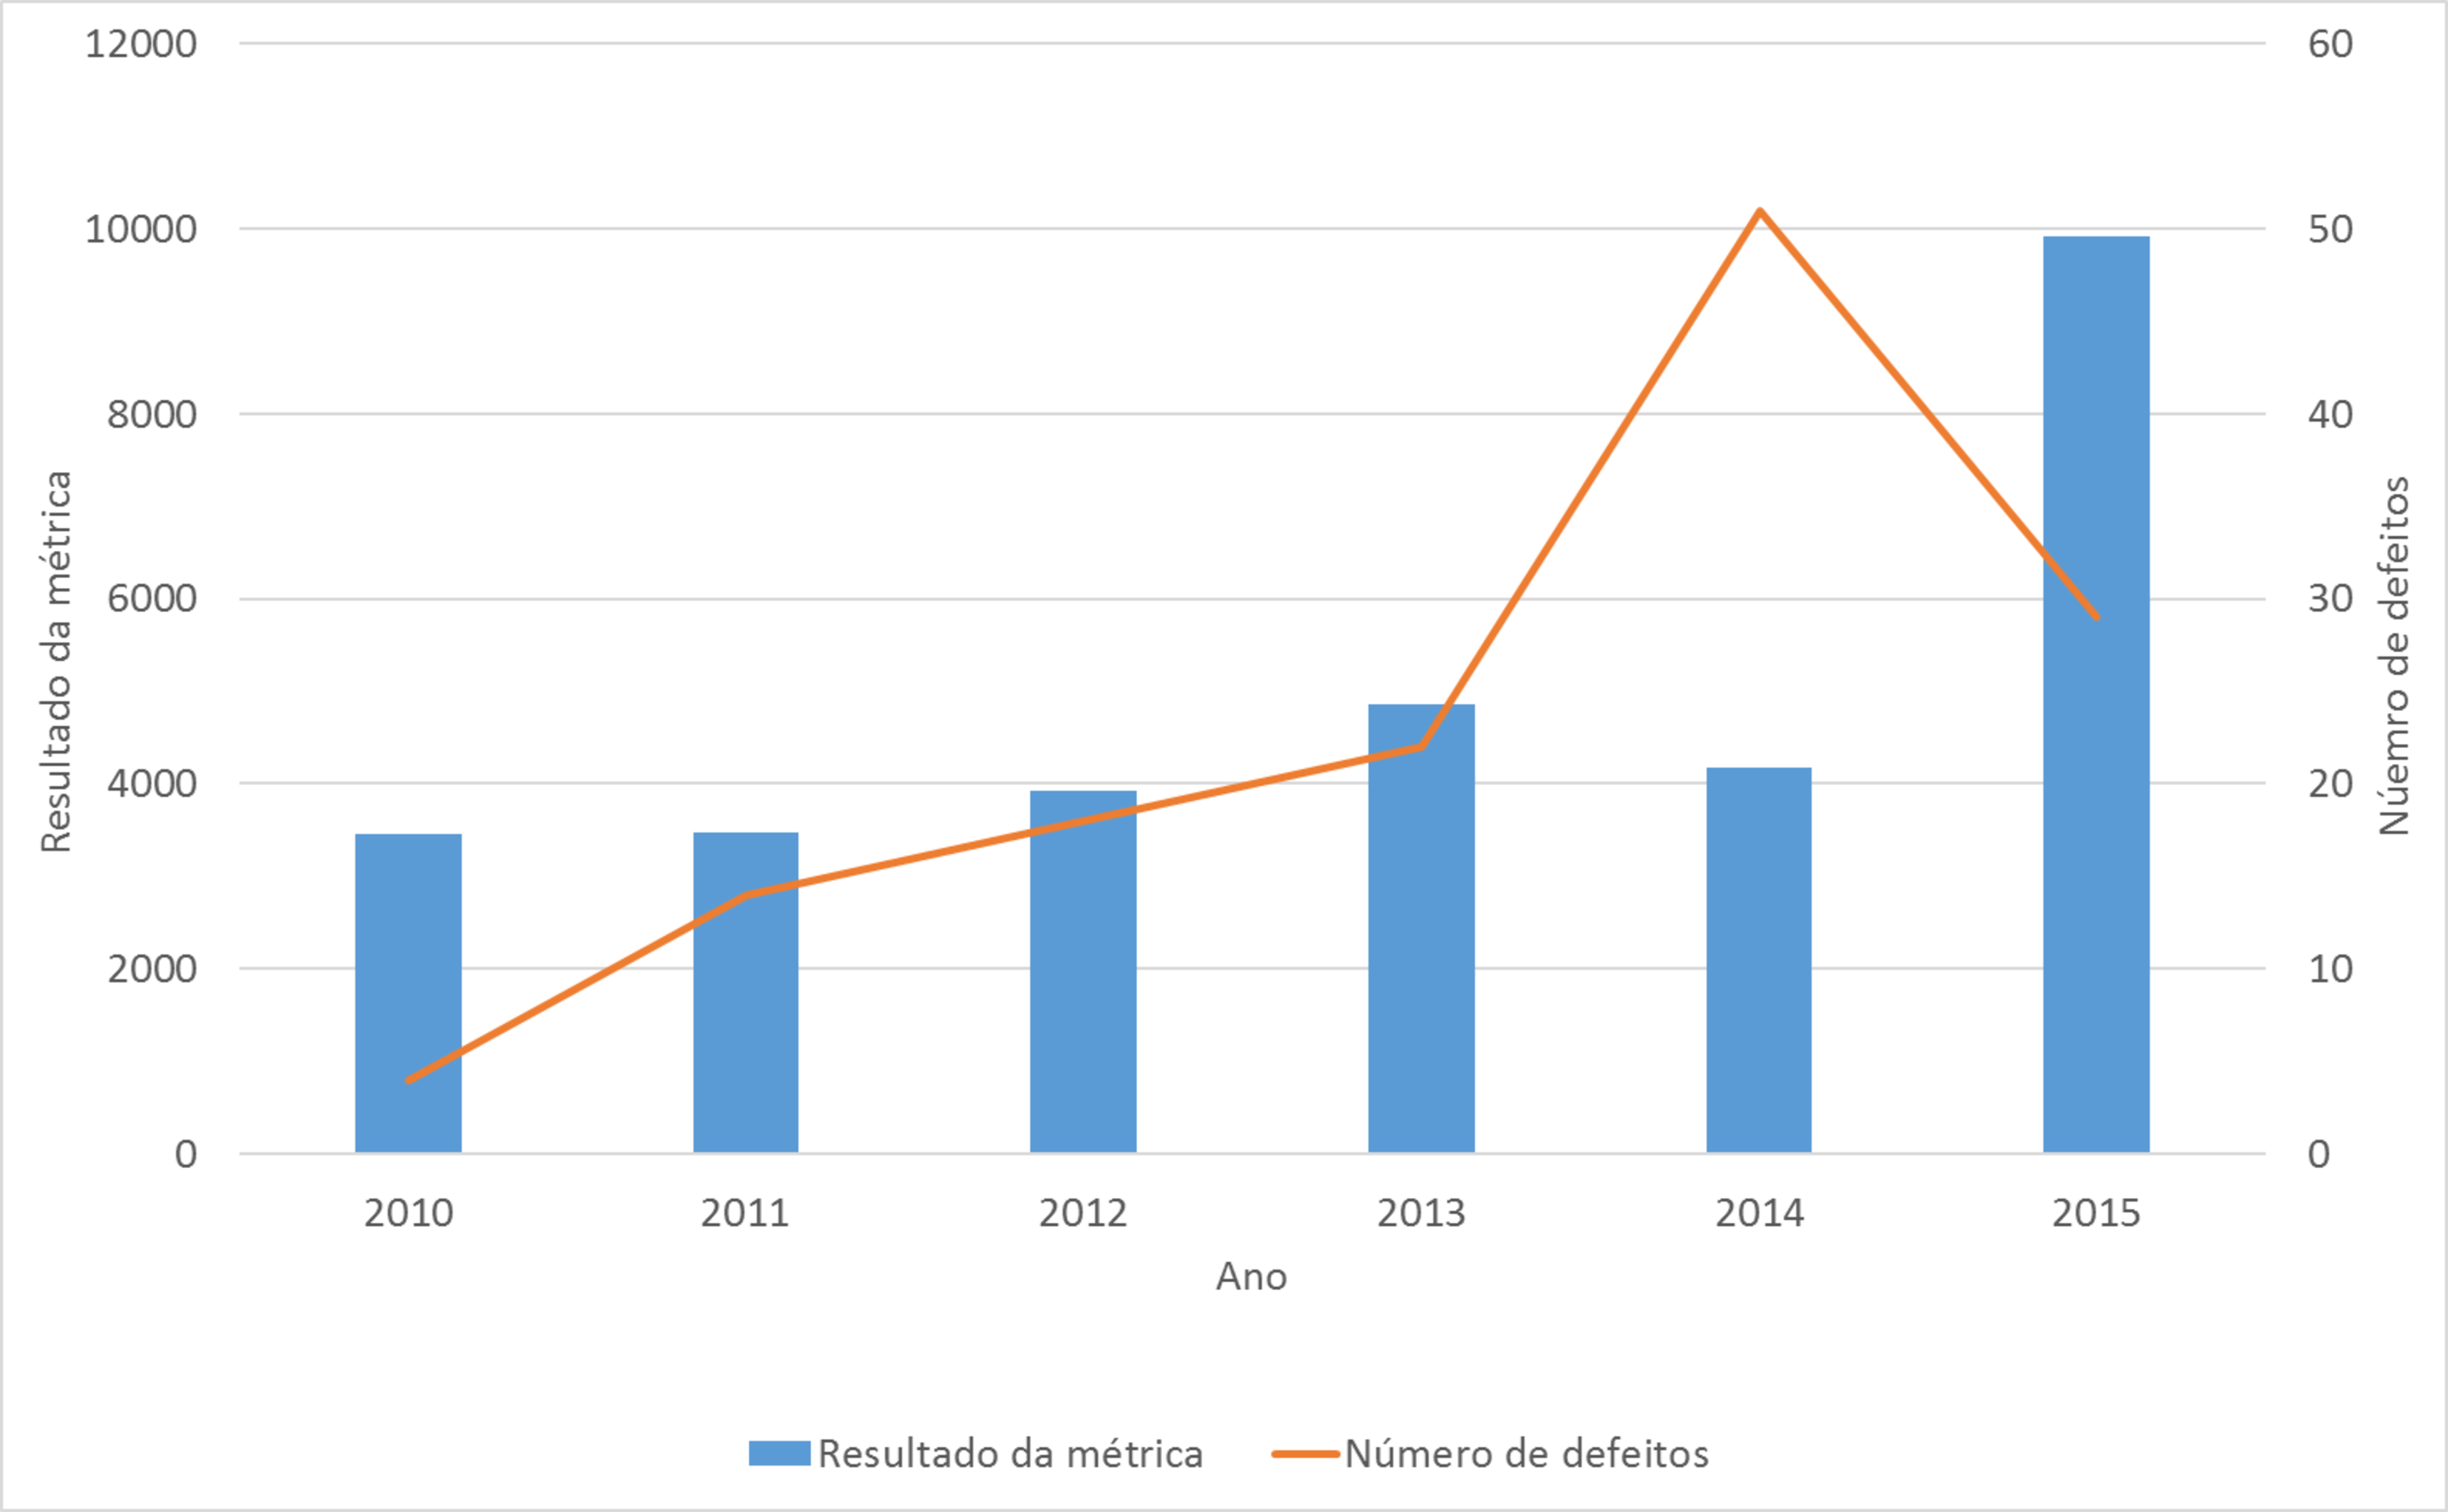
\includegraphics[width=1\textwidth]{./04-figuras/total_issues}
	\fonte{Próprio autor}
	\label{fig:totalXIssue}
\end{figure}

Pode-se notar na \autoref{fig:totalXIssue} que o número de defeitos acompanha a progressão da métrica, mas o pico de cadastro de defeitos não se encontra no mesmo intervalo em que há um pico do resultado da métrica. Este comportamento pode ser explicado pelo fato do \textit{layout} da aplicação ter sofrido uma mudança drástica entre as versões 1.549 e 1.574, disponibilizadas respectivamente em Janeiro/2014 (26/01/2014) e Julho/2014 (27/07/2014).

As folhas de estilo da biblioteca YUI representaram a maior porção do resultado total da métrica em grande parte das versões e também apresentou pouca mudança ao longo do tempo. Considerou-se, então, a possibilidade de isolar uma folha de estilo para análise do resultado, partindo do pressuposto que as modificações feitas pela equipe de desenvolvimento são as que impactam e definem a complexidade de manutenção do código. Para tanto foi necessária uma pesquisa no histórico de \textit{commits} dos arquivos CSS do projeto, com intuito de identificar que arquivos CSS haviam sofrido o maior número de alterações ao longo do tempo. Como pode ser visto na \autoref{tab:commits}, o arquivo \texttt{style.css} foi, excepcionalmente, o que sofreu mais \textit{commits}, sendo identificado, assim, como o arquivo de codificação CSS principal do projeto.

\begin{table}[!htbp]
	\centering
	\caption{Número de commits para cada arquivo CSS renderizado na página princpal do Jenkins.}
	\label{tab:commits}
	\begin{tabular}{l|c}
		\textbf{Arquivo CSS} & \textbf{Número de commits} \\ \hline
		style.css            & 113                        \\
		color.css            & 2                          \\
		responsive-grid.css  & 2                          \\
		yui\textbackslash button.css       & 3                          \\
		yui\textbackslash container.css    & 3                          \\
		yui\textbackslash menu.css         & 3                         
	\end{tabular}
\end{table}

A partir dessa identificação, a análise sobre progressão dos resultados e o número de defeitos criados foi refeita considerando somente o arquivo \texttt{style.css}, com o intuito de determinar o impacto das modificações feitas na folha de estilo principal do projeto sobre o número de defeitos.

\begin{figure}[!htb]
	\centering
	\caption{Comparação do resultado da métrica do \texttt{style.css} em relação ao número de defeitos criados.}
	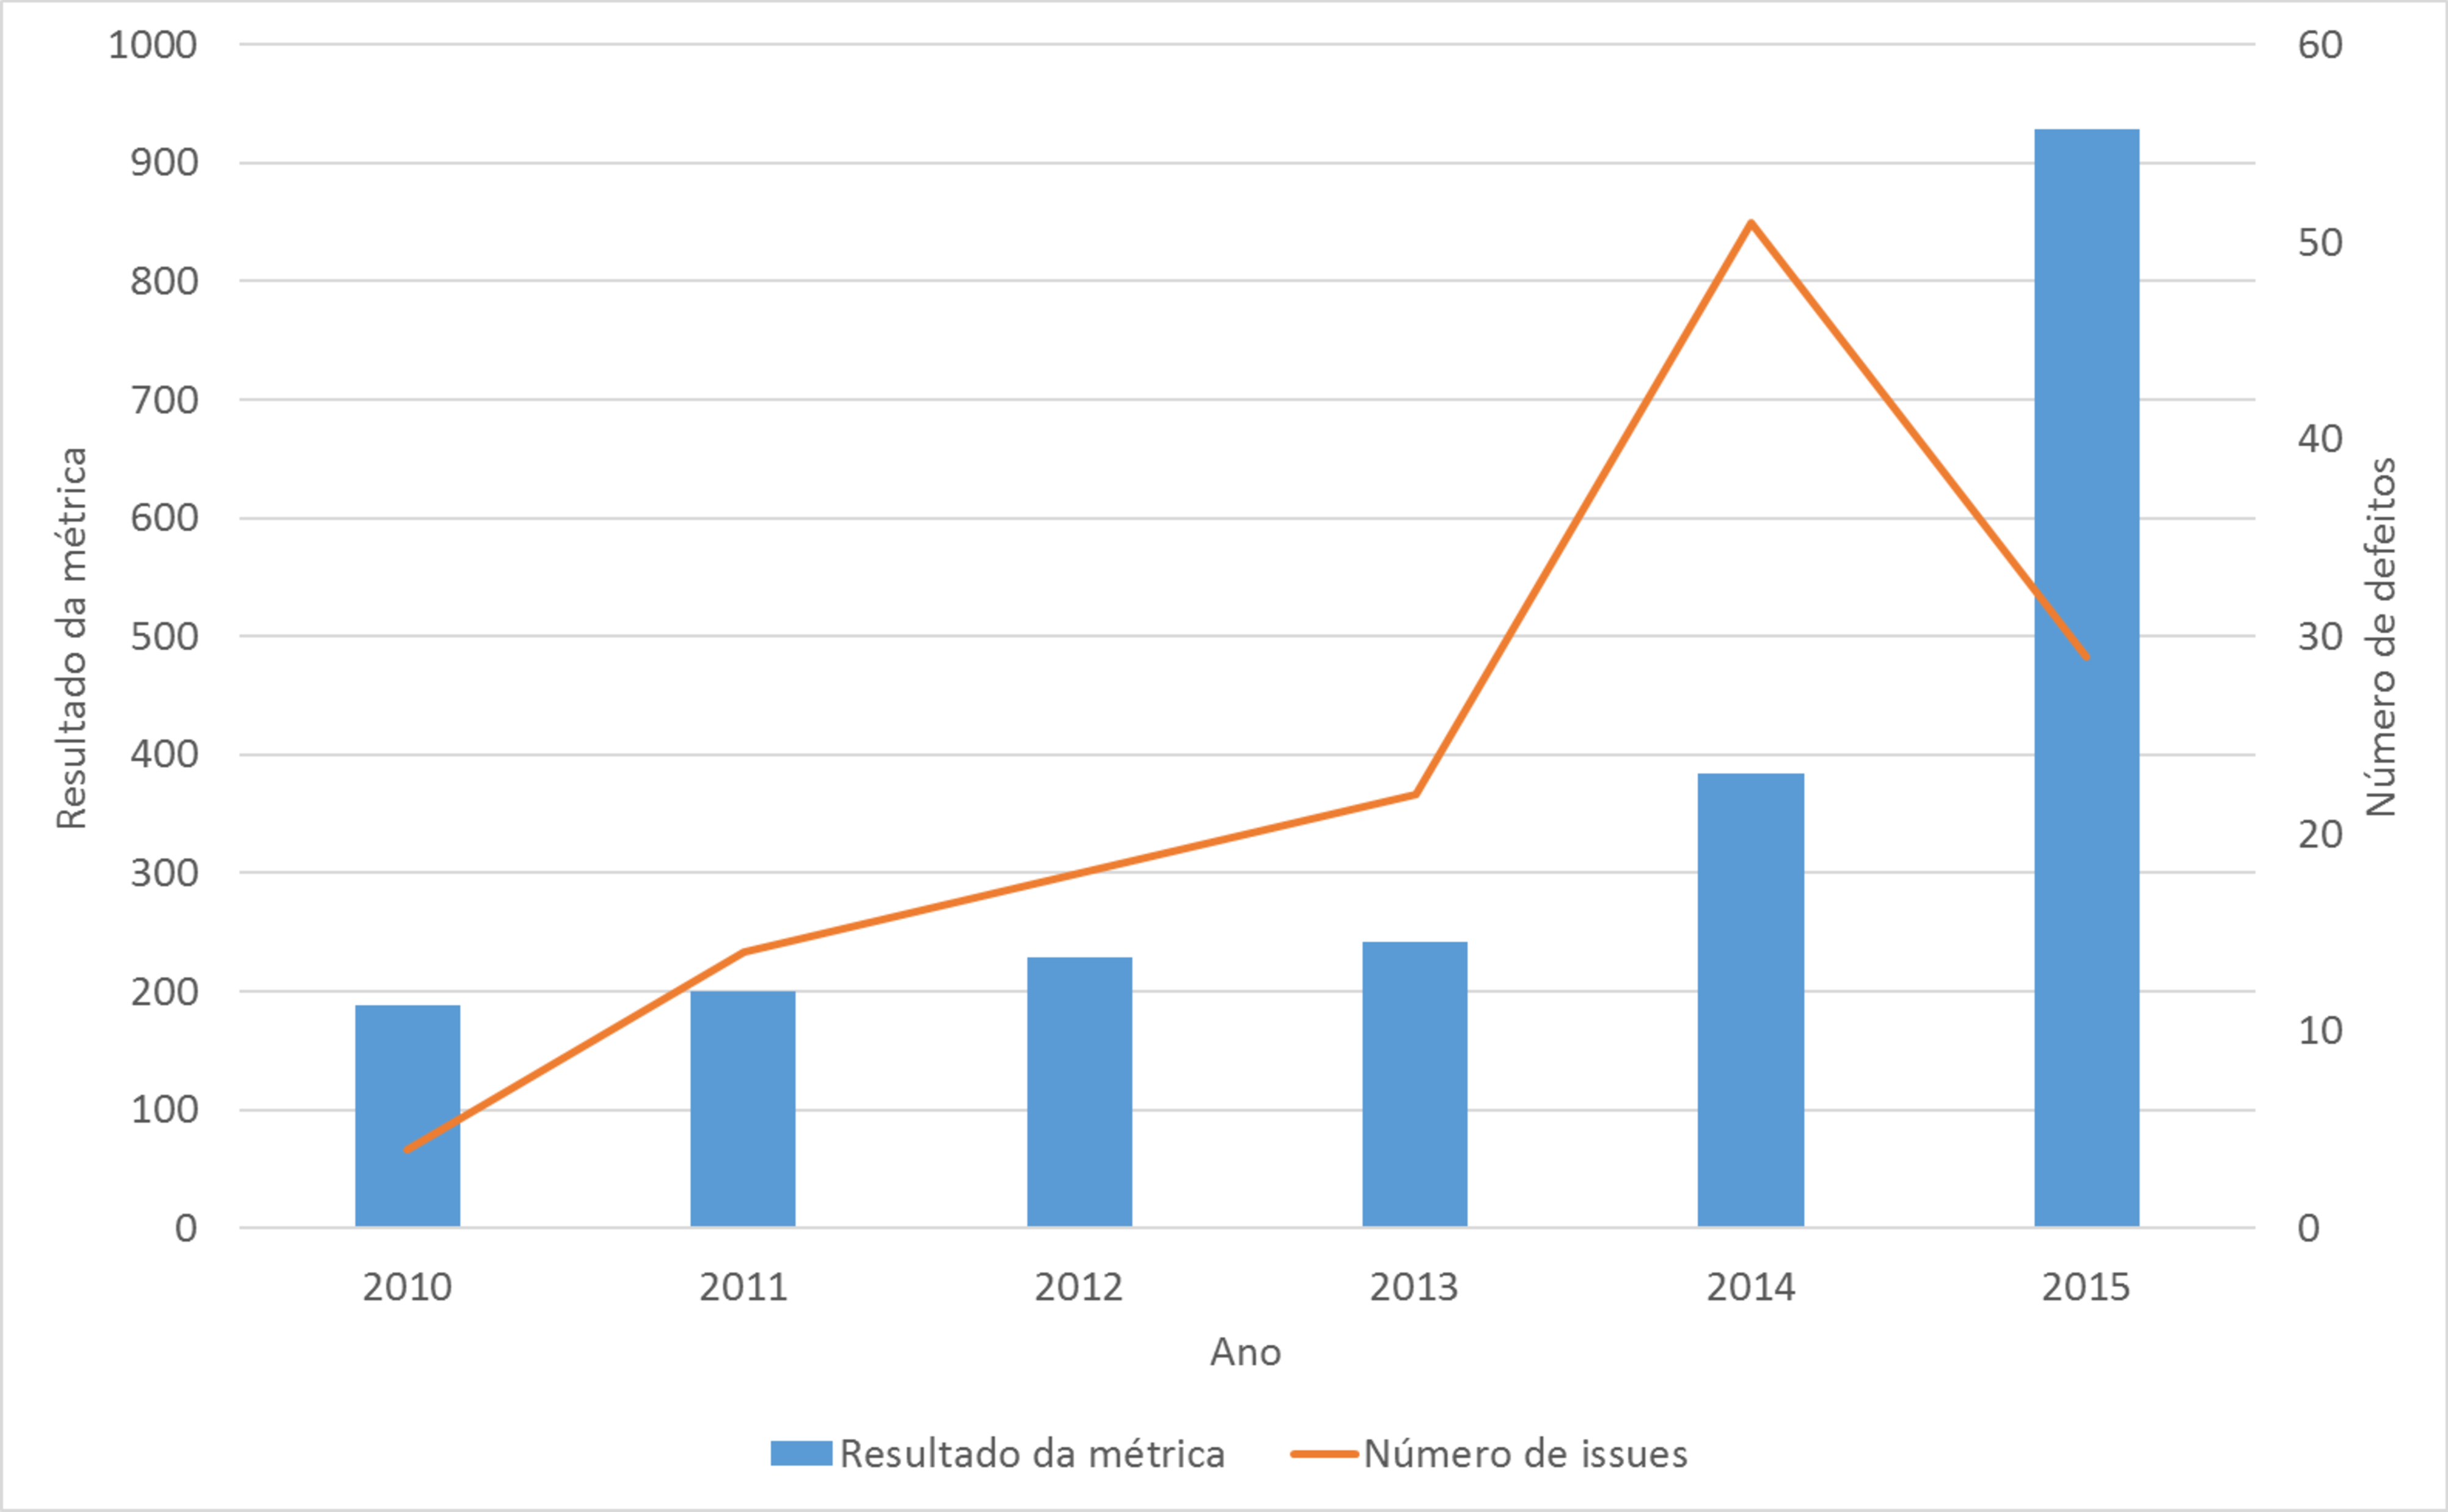
\includegraphics[width=0.9\textwidth]{./04-figuras/style_issues}
	\fonte{Próprio autor}
	\label{fig:styleXIssues}
\end{figure}

Pode-se notar na \autoref{fig:styleXIssues} que a evolução da métrica foi crescente durante toda a progressão temporal e também um aumento considerável do resultado referente à mudança de \textit{layout} em 2014.
%explicar melhor o agregado
O comportamento do resultado da métrica para somente o arquivo \texttt{style.css} e o somatório de todos os arquivos (\autoref{fig:totalXIssue}) é semelhante, o que leva a acreditar que o valor da métrica está relacionado às modificações feitas no projeto. Este comportamento para o arquivo \texttt{style.css} leva à hipótese de que as mudanças na folha de estilo causaram um aumento progressivo no resultado, ou seja, toda nova modificação somou ao valor da métrica.

Essa hipótese põe em questão qual o motivo desta mudança, que deve ser respondida através do estudo da métrica. Sobre quais são os critérios de avaliação que impactam no seu resultado e como esses se comportam. 

\section{Apreciação da Métrica}

Com o objetivo de avaliar a contribuição de cada critério no resultado final da métrica, fez-se uma análise da distribuição dentro do total de cada resultado. Na \autoref{fig:compos_crit}, pode-se notar uma variação em função do tempo na parcela de contribuição dos critérios. Essa variação pode ser originada a partir da necessidade de se corrigir as regras, ou adicionar novas, para cada uma das situações encontradas durante o período de manutenção.

%mudar a legenda

\begin{figure}[!htb]
	\centering
	\caption{Composição do valor da métrica por cada critério.}
	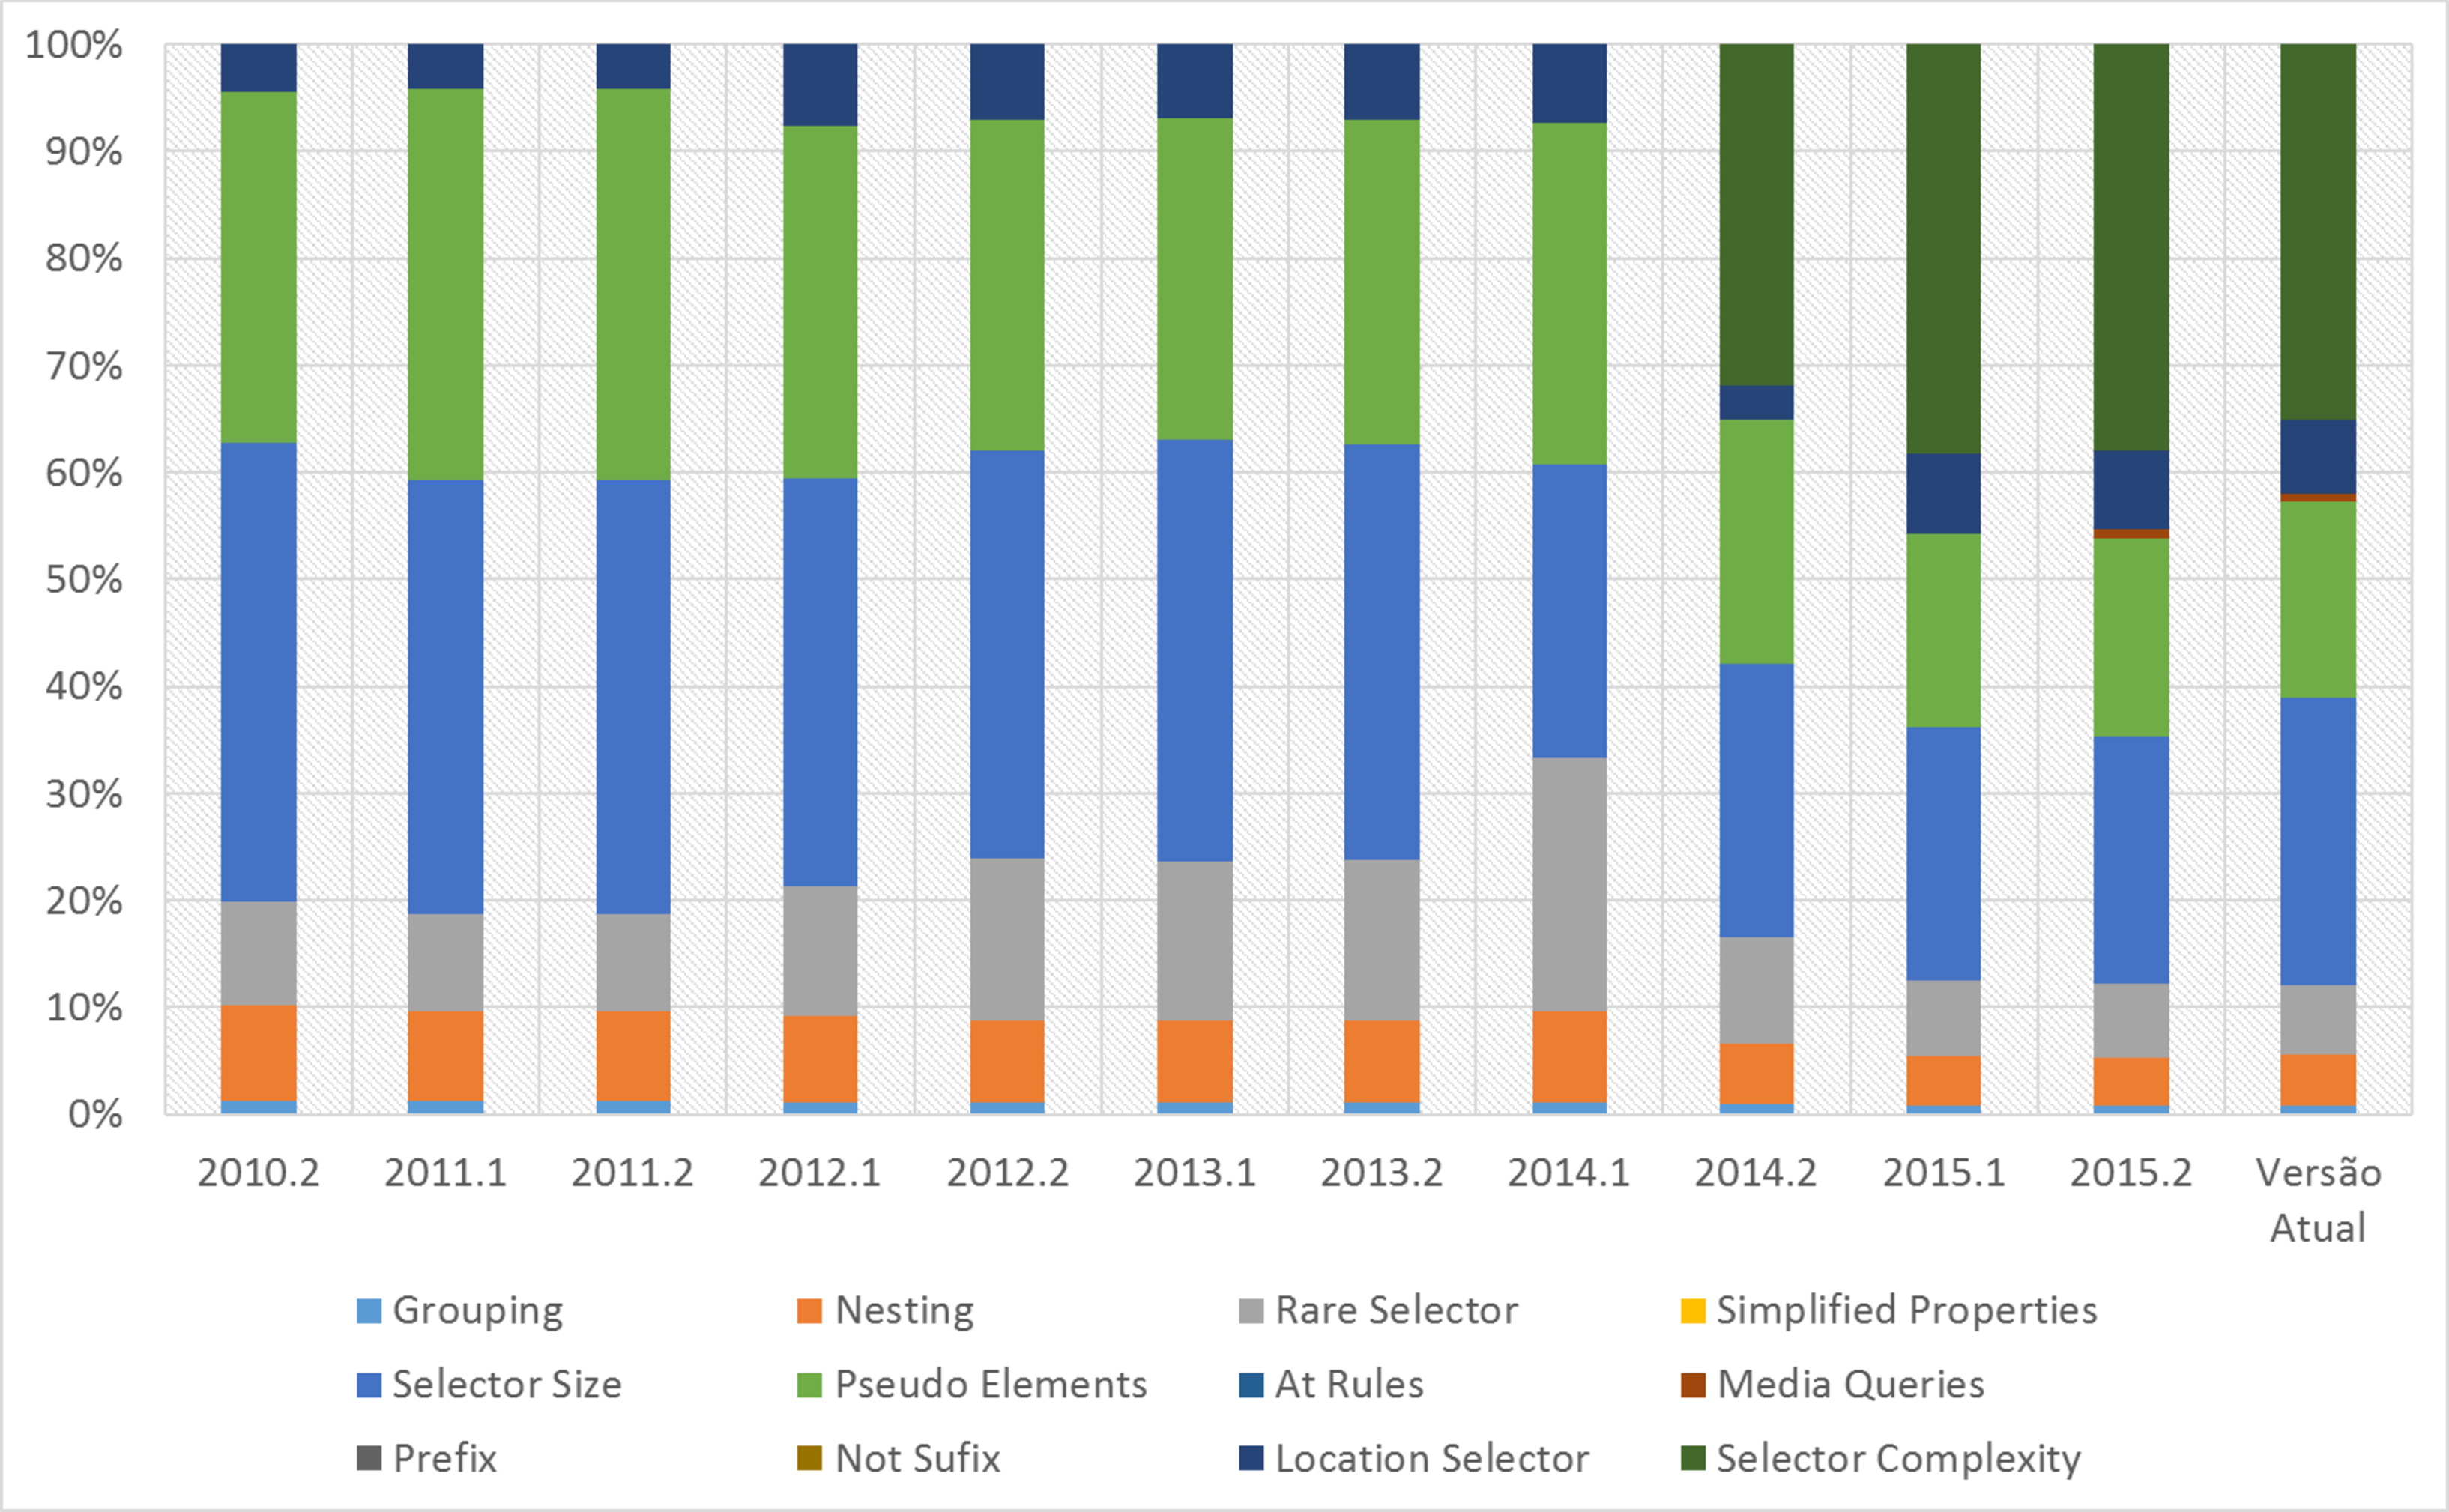
\includegraphics[width=0.9\textwidth]{./04-figuras/composition_criteria}
	\fonte{Próprio autor}
	\label{fig:compos_crit}
\end{figure}

O aumento da distribuição dos critérios de avaliação no resultado da métrica, pode ser interpretado como um aumento na complexidade do código.  Através da \autoref{fig:compos_crit}, nota-se que o perfil de complexidade foi se alterando com a evolução do código, o que pode ser explicado pelo aumento da contribuição ou o surgimento de outros critérios que antes não estavam presentes na avaliação da métrica.

Esse aumento de complexidade do código CSS pode ser um agente causador de efeitos colaterais que, por sua vez, podem causar um aumento considerável no número de defeitos no estilo de uma página \textit{web}. Esse fato pode explicar o aumento gradativo dos números de defeitos criados acompanhando o resultado da métrica, visto na \autoref{fig:styleXIssues}.

Os resultados obtidos nos testes demonstram um aumento de complexidade do código ao longo do tempo, sendo que essa complexidade impacta no número de defeitos encontrados. Porém, os resultados obtidos não são determinantes, por falta de uma base de comparação. Pode-se concluir, então, que a métrica apresentada é um passo importante em direção à definição de qualidade de código CSS e pode ser usada como base de comparação para investigações mais profundas de outras aplicações.